%%%%%%%%%%%%%%%%%%%%%%%%%%%%%%%%%%%%%%%%%%%%%%%%%%%%%%%%%%%%%%%%%%%%%%%%%%%%%%%
% i7 Seminar Report Template
% Version November 8, 2023

\documentclass[a4paper,11pt,DIV=14]{scrartcl} % Do not edit this line.


%%%%%%%%%%%%%%%%%%%%%%%%%%%%%%%%%%%%%%%%%%%%%%%%%%%%%%%%%%%%%%%%%%%%%%%%%%%%%%%
% Preamble

% Page Geometry, Typography and Encoding
\usepackage[utf8]{inputenc}
\usepackage[T1]{fontenc}
\usepackage{microtype}
\usepackage{lmodern}
\renewcommand{\phi}{\varphi}
\renewcommand{\epsilon}{\varepsilon}
% \renewcommand{theta}{\vartheta} % if you want

% \usepackage[textwidth=426p]{geometry}

% Math packages
\usepackage{amsmath}
\usepackage{amssymb}
\usepackage{amsthm}
\usepackage{mathtools}

% Floats
\usepackage{float}
\usepackage{booktabs}
\usepackage{tikz}
\usetikzlibrary{positioning,arrows.meta}

% Colors
\usepackage{xcolor} %already loaded by tikz, but here for completeness
% RWTH colors
% blue violet purple carmine red magenta orange yellow grass cyan gold silver
\definecolor{rwth-blue}{cmyk}{1,.5,0,0}\colorlet{rwth-lblue}{rwth-blue!50}\colorlet{rwth-llblue}{rwth-blue!25}
\definecolor{rwth-violet}{cmyk}{.6,.6,0,0}\colorlet{rwth-lviolet}{rwth-violet!50}\colorlet{rwth-llviolet}{rwth-violet!25}
\definecolor{rwth-purple}{cmyk}{.7,1,.35,.15}\colorlet{rwth-lpurple}{rwth-purple!50}\colorlet{rwth-llpurple}{rwth-purple!25}
\definecolor{rwth-carmine}{cmyk}{.25,1,.7,.2}\colorlet{rwth-lcarmine}{rwth-carmine!50}\colorlet{rwth-llcarmine}{rwth-carmine!25}
\definecolor{rwth-red}{cmyk}{.15,1,1,0}\colorlet{rwth-lred}{rwth-red!50}\colorlet{rwth-llred}{rwth-red!25}
\definecolor{rwth-magenta}{cmyk}{0,1,.25,0}\colorlet{rwth-lmagenta}{rwth-magenta!50}\colorlet{rwth-llmagenta}{rwth-magenta!25}
\definecolor{rwth-orange}{cmyk}{0,.4,1,0}\colorlet{rwth-lorange}{rwth-orange!50}\colorlet{rwth-llorange}{rwth-orange!25}
\definecolor{rwth-yellow}{cmyk}{0,0,1,0}\colorlet{rwth-lyellow}{rwth-yellow!50}\colorlet{rwth-llyellow}{rwth-yellow!25}
\definecolor{rwth-grass}{cmyk}{.35,0,1,0}\colorlet{rwth-lgrass}{rwth-grass!50}\colorlet{rwth-llgrass}{rwth-grass!25}
\definecolor{rwth-green}{cmyk}{.7,0,1,0}\colorlet{rwth-lgreen}{rwth-green!50}\colorlet{rwth-llgreen}{rwth-green!25}
\definecolor{rwth-cyan}{cmyk}{1,0,.4,0}\colorlet{rwth-lcyan}{rwth-cyan!50}\colorlet{rwth-llcyan}{rwth-cyan!25}
\definecolor{rwth-teal}{cmyk}{1,.3,.5,.3}\colorlet{rwth-lteal}{rwth-teal!50}\colorlet{rwth-llteal}{rwth-teal!25}
\definecolor{rwth-gold}{cmyk}{.35,.46,.7,.35}
\definecolor{rwth-silver}{cmyk}{.39,.31,.32,.14}

% Hyperlinks and Cross-References
\usepackage{hyperref}
\usepackage[capitalise,noabbrev]{cleveref}
\hypersetup{%
	pdftoolbar=false,
	pdfmenubar=false,
	colorlinks,
	%pdfborderstyle={/S/U/W 1.25},
	urlcolor={rwth-magenta},
	linkcolor={rwth-red},
	citecolor={rwth-green}
}



\theoremstyle{plain}
\newtheorem{theorem}{Theorem}[section]
\newtheorem{proposition}[theorem]{Proposition}
\newtheorem{lemma}[theorem]{Lemma}
\newtheorem{corollary}[theorem]{Corollary}
\newtheorem{conjecture}[theorem]{Conjecture}
\newtheorem{claim}[theorem]{Claim}
\theoremstyle{definition}
\newtheorem{definition}[theorem]{Definition}
\newtheorem{remark}[theorem]{Remark}


% Misc packages
\usepackage{lipsum}

\usepackage{tikz}
\usetikzlibrary{automata, positioning, arrows, calc, fit, shapes.misc}

\usepackage{multicol}

\usepackage{todonotes}

\usepackage{subcaption}

% Custom commands
\newcommand{\GFC}{\mathsf{GF}(\mathsf{C})}
\newcommand{\free}[1]{\operatorname{free}(#1)}
\newcommand{\gd}[1]{\operatorname{gd}(#1)}
\newcommand{\RCR}{\operatorname{RCR}}
\newcommand{\CR}{\operatorname{CR}}
\newcommand{\disjunctiveGFC}{\operatorname{disjunctive-\GFC}}
\newcommand{\set}{\operatorname{set}}
\newcommand{\ipo}{i+1\operatorname{mod}}
\newcommand{\Hom}{\operatorname{Hom}}
\newcommand{\C}[1]{\mathsf{C}_{#1}}
\newcommand{\atp}{\operatorname{atp}}
\newcommand{\stp}{\operatorname{stp}}

\renewcommand{\theta}{\vartheta}
\renewcommand{\rho}{\varrho}

\newcommand{\term}[1]{\operatorname{\textit{#1}}}

\def\multiset#1{\ensuremath{\left\{\kern-.35em\left\{#1\right\}\kern-.35em\right\}}}
\newcommand{\leftmultiset}{\ensuremath{\{\kern-.35em\{}}
\newcommand{\rightmultiset}{\ensuremath{\}\kern-.35em\}}}

%%%%%%%%%%%%%%%%%%%%%%%%%%%%%%%%%%%%%%%%%%%%%%%%%%%%%%%%%%%%%%%%%%%%%%%%%%%%%%%
% Document


\begin{document}

%TODO Insert topic of seminar, e.g. Theoretical Topics in Data Science or Complexity Theory
\subtitle{Bachelor's Thesis}
\date{August 28, 2025}
\publishers{RWTH Aachen University}	% Do not edit this line.

%TODO Change this to your report title.
\title{Relational Colour Refinement for Non-Relational Signatures}

%TODO Change this to your name.
\author{Theodor Jurij Teslia}

\maketitle

%TODO Provide a short abstract for your report.
\begin{abstract}
	Colour Refinement is an iterative graph algorithm that computes a colouring of the vertices, based on the colouring of their direct neighbours.
	Aside from useful applications in various fields, it is theoretically interesting, due to its characterisations.
	It was proved that the distinguishing power of Colour Refinement is equivalent to that of counting logic with two variables and to that of counting homomorphisms from trees.
	Therefore, the question, whether such an algorithm is also possible for extensions of graphs was posed.
	Recently, Scheidt and Schweikardt defined an algorithm for relational structures with analogous properties.
	Especially the characterisations are similar to classical Colour Refinement.
	As such, its distinguishing power is equivalent to that of the guarded fragment of counting logic and to that of counting homomorphisms from $\alpha$-acyclic relational structures.
	
	In this thesis, we want to present the results of Scheidt and Schweikardt and investigate the robustness of their algorithm and characterisations.
	Concretely, we consider extending the class of relational structures to that of all structures and of structures with relations and unary functions, respectively.
	We find two logical characterisations but disprove the existence of a characterisation through homomorphism counting.
	Furthermore, we discuss for which restrictions on relational structures the characterisation through homomorphism counting remains and present two cases of restrictions, one for which the characterisation holds and one for which it does not.
\end{abstract}

\thispagestyle{empty}

\clearpage

%TODO The content of your report gos below.

\section{Introduction}

The graph isomorphism problem is a very interesting and important problem in both theoretical and applied computer science.
The question, whether two graphs are structurally identical comes up in many fields of research.
For example when trying to recognize identical chemical structures for patent verification \cite{ray1957FindingChemical} or finding symmetries for optimizing problems such as the Boolean Satisfiability problem \cite{grohe2020GraphIsomorphism}.
Furthermore, the graph isomorphism problem is interesting from a complexity theoretic perspective, as it is a prominent example for a problem, which has not been proven to be either $\mathsf{NP}$-complete or solvable in polynomial time. \cite{babai2016GraphIsomorphism}

One (incomplete) algorithm that is often used in practical isomorphism problem solvers \cite{grohe2020GraphIsomorphism} is \emph{Colour Refinement}, short $\CR$, also called the \emph{1-dimensional Weisfeiler-Leman algorithm}.
Given two graphs, it can prove in quasilinear time that they are not isomorphic \cite{berkholz2017TightLowera}.
Concretely, $\CR$ is an iterative algorithm that, in the beginning, assigns every vertex the same colour and in following iterations assigns each one a new colour, based on the colours of its neighbours.
This procedure is repeated, until the partition of the vertices induced by the colouring stays the same. 
We then say that Colour Refinement distinguishes two graphs, if there is some colour that appears differently often in the two graphs.
It is easy to see that two isomorphic graphs are not distinguished by Colour Refinement.
This is equivalent to the fact that if two graphs get distinguished by Colour Refinement, then they cannot be isomorphic.
Furthermore, while it is not possible to infer the opposite direction, that is two non-isomorphic graphs always get distinguished by $\CR$, it was shown by Babai, Erd\H{o}s and Selkow that almost all graphs get distinguished by it \cite{babai1980RandomGraph}.
However, there exist some classes of graphs, that cannot be distinguished by Colour Refinement, for example the classes of regular graphs with the same number of vertices.

Aside from isomorphism testing, Colour Refinement has applications in different fields.
Incidentally, the first recorded occurrence of this algorithm appeared in 1965 and dealt with the description of chemical structures \cite{morgan1965GenerationUnique}.
Its significance for computer science has been recognised later by Weisfeiler and Leman in 1968 \cite{weisfeiler1968reduction}.
One interesting application of Colour Refinement is in the reduction of the dimension of linear programs.
By defining a variant of Colour Refinement on matrices which finds a partition of the rows and columns, it is possible to reformulate a linear program with a considerably smaller dimension. 
This method of first reducing the problem and then solving the reduced instance has been shown to be more performant than the standard way of solving linear programs. \cite{grohe2014DimensionReduction}
Another application can be found in the field of machine learning, more precisely for kernel methods.
Generally, the aim of kernel methods is to assign a similarity value between two elements, which then can be used in more complex machine learning techniques such as support vector machines or regression.
An emerging concept in this field are kernels for graphs, also called graph kernels, which are a method to compare two graphs, and represent how similar they are with a single value.
Standard graph kernel methods consider certain subgraphs and count the (dis-)similarities. \cite{vishwanathan2010graph}
One interesting application of Colour Refinement can be found in its usage as a graph kernel.
When fixating an integer $h$ and counting for each of the first $h$ Colour Refinement steps how many vertices between two graphs share the same colour, we get a graph kernel.
This Weisfeiler-Leman Graph Kernel has an adequate ability to to classify graphs, while having a significantly better runtime than classical graph kernels. \cite{grohe2021ColorRefinement}

The importance of $\CR$ in theoretical computer science can be seen, when  we consider other characterisations of its distinguishing power.
Thus, $\CR$ can be equivalently characterised by counting homomorphisms from trees and by considering a certain logic.
Due to Dvo\v r\'ak \cite{dvorak2010RecognizingGraphsa} and Dell, Grohe and Rattan \cite{dell2018LovaszMeets} we have the following characterisation.
Given two graphs $G$ and $H$, we have that Colour Refinement distinguishes them if, and only if, there is some tree $T$ such that the number of homomorphisms from $T$ to $G$ is different than to $H$.
Such a characterisation can also be done through logic.
We define $\C{2}$ as the logic that extends first-order logic by counting quantifiers and only uses up to two variables.
Then, it was the shown by Cai and Immerman \cite{cai1992OptimalLower} and Immerman and Lander \cite{immerman1990DescribingGraphs} that the following holds: 
Colour Refinement distinguishes $G$ and $H$ if, and only if, there is a sentence $\phi\in\C{2}$ such that $G\models \varphi$ and $ H\not\models \varphi$.

From the above examples it can be seen that while Colour Refinement is a simple procedure, it can be applied in various situations.
This versatility has been one of the reasons for its success and poses the question, whether it could be possible to formulate an analogous procedure for more than graphs.
One obvious extension of graphs are hypergraphs.
These are structures with a set of vertices and edges between those.
However, while the edges of classical graphs connect two vertices, edges of hypergraphs can include an arbitrary number of them.
One interesting result due to Böker \cite{boker2019ColorRefinement} is an extension of Colour Refinement to hypergraphs, which gives rise to an analogous characterisation using homomorphism counting.
Concretely, Colour Refinement for a hypergraph $G$ is defined like classical $\CR$ on a coloured variant of the incidence graph of $G$.
We then consider connected Berge-acyclic hypergraphs, that is hypergraphs whose incidence graphs are trees. 
When counting homomorphisms from those to hypergraphs, we get that Colour Refinement distinguishes two hypergraphs $G$ and $H$ if, and only if, there is some connected Berge-acyclic hypergraph $B$, such that $B$ has a different number of homomorphisms to $G$ than to $H$.
Another result with respect to hypergraphs has been achieved by Scheidt and Schweickardt in \cite{scheidt2023CountingHomomorphisms}.
They devised a 2-sorted counting logic called $\mathsf{GC}^k$ and proved that two hypergraphs $G$ and $H$ satisfy exactly the same $\mathsf{GC}^k$ sentences if, and only if, all hypergraphs with generalised hypertree width $k$ have the same number of homomorphisms to $G$ as to $H$.
For the case where $k=1$, we then get indistinguishability over the class of all $\alpha$-acyclic hypergraphs, which is a strictly stronger measure of acyclicity than Berge-acyclicity.
Interestingly, we will encounter $\alpha$-acyclicity and $\mathsf{GC}^1$ in section \ref{sec:RelationalColourRefinement} for characterising relational structures, instead of hypergraphs.
A first effort to extend Colour Refinement to relational structures has been made by Butti and Dalmau in \cite{butti2021FractionalHomomorphism}.
They also defined Colour Refinement on the incidence graph of a relational structure and proved that this distinguishes two relational structures if, and only if, there is a connected Berge-acyclic relational structure with a different number of homomorphisms to the structures.
A more recent result with respect to relational structures has been made by Scheidt and Schweikardt \cite{scheidt2025ColorRefinement}.
They defined an extension of Colour Refinement for relational structures, called Relational Colour Refinement, short $\RCR$, which is stronger than the version in \cite{butti2021FractionalHomomorphism}.
Thus it can distinguish structures that the variant in \cite{butti2021FractionalHomomorphism} cannot.
Furthermore, they were able to define the logic $\GFC$, which characterises $\RCR$ in the same way as $\C{2}$ characterises classical $\CR$.
Additionally, the aforementioned $\alpha$-acyclic structures characterise $\RCR$ as well.
Concretely, we have that two relational structures of the same signature get distinguished by $\RCR$ if, and only if, there is an $\alpha$-acyclic structure of the same signature such that is has a different amount of homomorphisms to the structures.
A deeper discussion of the results from \cite{scheidt2025ColorRefinement} can be found in section \ref{sec:RelationalColourRefinement}.

% Abschnitt nicht so überzeugend
% Motivation für das fehlt, "gibt für rel struc und hypergraph"
% Warum Interesse an funktionalen Signaturen
% Fragestellung mot funktional auf beiden Seiten von iff. nicht klar
% Iwi zu technisch? Vllt auch nicht
% Text trennen:
% Paragraph: New results of this thesis
% Zentrale 2-3 Theoreme da staten: Wird klarer was sind die Ergebnisse
% In abgespeckt/verbaler um nicht ganze Notation einzuführen
% Thm 1 aus Intro vereinfachte Form von Thm x

It can be seen that Colour Refinement for graphs, as for relational structures and hypergraphs have been studied.
Especially the results from \cite{scheidt2025ColorRefinement} seem like a very robust and usable extension for relational structures.
Furthermore, we notice that functional, as well as non-relational signatures have not yet been investigated.
As many practical and useful structures use non-relational signatures, for example all algebraic structures, we pose the question how robust the results from \cite{scheidt2025ColorRefinement} are when using them with (unary) functions.
Concretely, we consider two possible ways of how Relational Colour Refinement can be adapted to signatures with functions.
For both approaches we investigate, whether they can be characterised by $\GFC$ over signatures with functions and by counting homomorphisms from acyclic structures with non-relational signatures.
We will see that such a characterisation through logic is in fact possible, while counting homomorphisms from acyclic structures is not.
Additionally, we prove a similar result to the (not existing) characterisations by counting homomorphisms.
We show that while it is not possible to require that the acyclic structure is functional (given a signature with functions), it is possible to require the acyclic structure to be symmetric (given that the two distinguished structures are symmetric as well).
Therefore, we get that two symmetric structures are distinguished by $\RCR$ if, and only if, there is some symmetric, acyclic structure with different numbers of homomorphisms to the structures.

The results of this thesis are as follows.
We define two variants of $\RCR$ for non-relational signatures, called naive $\RCR$ and $\RCR_k$ for a $k\in\mathbb{N}$, where the latter is only defined for unary functions.
Naive $\RCR$ encodes $n$-ary functions $f$ directly as a $(n+1)$-ary relations $R_f$, such that $(x_1,\dots,x_n,y)\in R_f$ if, and only if, $f(x_1,\dots,x_n)=y$ and then applies normal $\RCR$ to the relational structure.
$\RCR_k$ encodes unary functions $f$ as a family of relations $R_{f^1}$, $R_{f^2}$, $\dots$, where $(x,y)\in R_{f^i}$ if, and only if, $f^i(x)=y$, that is the $n$-times application of $f$ on $x$.
Furthermore we define $\mathsf{nfGF}(\mathsf C)$ as the logic that is defined as $\GFC$ over non-relational signatures but does not allow the nesting of terms. 
Additionally we define $\GFC_k$ as the logic that is the normal extension of $\GFC$ to non-relational signatures but terms are only allowed to have an alternation-depth of function-applications of $k$.
We then achieve the following results.

\textbf{Theorem \ref{thm:ThmA}}:
For a non-relational signature $\sigma$ and two $\sigma$-structures $\mathfrak A$ and $\mathfrak B$, we have that naive $\RCR$ distinguishes $\mathfrak A$ and $\mathfrak B$ if, and only if, there is a sentence $\phi\in \mathsf{nfGF}(\mathsf C)$ of signature $\sigma$ such that $\mathfrak A\models \phi$ and $\mathfrak B\not\models \phi$.

\textbf{Theorem \ref{thm:ThmB}}:
For a non-relational signature $\sigma$ that only contains relation-symbols and unary function-symbols, two $\sigma$-structures $\mathfrak A$ and $\mathfrak B$ and a $k\in\mathbb N$, we have that $\RCR_k$ distinguishes $\mathfrak A$ and $\mathfrak B$ if, and only if, there is a sentence $\phi\in \GFC_k$ of signature $\sigma$ such that $\mathfrak A\models \phi$ and $\mathfrak B\not\models \phi$.

\textbf{Theorem \ref{thm:nRCRNotCharacByHomCount}}:
There exist two families of structures $(\mathfrak A_i)_{i\in\mathbb N_{\geq 4}}$ and $(\mathfrak B_i)_{i\in\mathbb N_{\geq 4}}$ such that naive $\RCR$ distinguishes $\mathfrak A_i$ and $\mathfrak B_i$ for all $i\geq4$, but there does not contain an acyclic, total and functional structure that distinguishes $\mathfrak A_i$ and $\mathfrak B_i$ by number of homomorphism.

\textbf{Theorem \ref{thm:ThmD}}:
For two symmetric, relational structures $\mathfrak A$ and $\mathfrak B$, we have that $\RCR$ distinguishes $\mathfrak A$ and $\mathfrak B$ if, and only if, there is a symmetric, acyclic structure that distinguishes $\mathfrak A$ and $\mathfrak B$ by number of homomorphism.

The methods used to achieve the above results rely heavily on the proofs from \cite{scheidt2025ColorRefinement}.
For the logical characterisation of structures with functions we translate both structures to relational structures and translate any formula to a valid $\GFC$-formula over a relational signature.
The same is done in reverse as well.
For the characterisation through homomorphism counting we present two families of structures.
We prove that two structures from the families of the same size get distinguished by naive $\RCR$ but there cannot be an acyclic structure of the same signature such that it distinguishes them by homomorphism count.

The structure of this thesis is as follows.
We begin by defining notation and fundamental definitions in section \ref{sec:Preliminaries}.
Then in section \ref{sec:RelationalColourRefinement} we present and explain the results from \cite{scheidt2025ColorRefinement}.
Afterwards, we continue in section \ref{sec:RelationalColourRefinemetForStructuresWithFunctions} by considering structures with functions, where we will first show the logical characterisation for the two approaches, before then presenting the family of counterexamples for the characterisation through homomorphism counting.
Lastly, we discuss the restriction to symmetric structures in section \ref{sec:RelationalColourRefinementForSymmetricStructures}.

% Erst Intro noch fertig machen
% Dann Beweise am Ende fertig
% Dann Kapitel 2 und 3


% Ende nächster Woche schicken was ich habe



\section{Preliminaries}
\label{sec:Preliminaries}

% Tuple notation
Let $A$ be a set.
Then a $a_1,\dots, a_k\in A$ form a tuple with length $k$ of the form $\mathbf a=(a_1,\dots,a_k)\in A^k$ and with $\mathbf a_n$ we denote $a_n$.
For any function $f:A\to B$, we write $f(\mathbf a)$ for $(f(a_1),\dots,f(a_k))$.
If $\pi$ is a permutation, that is $\pi\in \mathcal S_k$, where $\mathcal S_k$ is the symmetric group for $k$ elements, then $\pi(\mathbf a)$ means $(a_{\pi(1)},\dots,a_{\pi(k)})$.
For a set $A$ and a $k\in \mathbb N$, we write $\binom{A}{k}$, to denote all subsets of $A$ with cardinality of exactly $k$.
Let $\mathbf a=(a_1,\dots,a_k)\in A^k$ be a tuple of length $k$ and $b\in A$.
Then we write $(\mathbf ab)\coloneqq(a_1,\dots,a_k,b)$ for the tuple of length $k+1$ with $b$ added to the end.
For a tuple $\mathbf a=(a_1,\dots,a_k)$ we write $\set(\mathbf a)\coloneqq\{a_1,\dots,a_k\}$ for the set that contains the elements from $\mathbf a$.
Usually, sets are denoted by uppercase, elements from sets as lowercase, and tuples as boldface and lowercase Latin letters.

% Natural numbers
By $\mathbb N$ we mean the set of natural numbers, including $0$, and with $\mathbb N_{\geq k}$ for a $k\in \mathbb N$, we denote the set $\{k,k+1,\dots\}=\mathbb N \setminus \{0,\dots,k\}$.
We use $[k]$ for any $k\in \mathbb N_{\geq 1}$ to mean $\{1,2,\dots, k\}$.

% Multisets
A multiset $\mathcal M$ is a pair with a set $A$ and a function $\operatorname{mult}_{\mathcal M}:A\to \mathbb N_{\geq 1}$.
This denotes, that for every $a\in A$, there are exactly $\operatorname{mult}_{\mathcal M}(a)$ many copies in $\mathcal M$.
We also write multisets as $\multiset{\dots}$.
As an example, the multiset $\mathcal M = \multiset{a, b, b}$ is equivalent to the set $A=\{a,b\}$, together with the function $\operatorname{mult}_{\mathcal M}=\{a\mapsto 1, b\mapsto 2\}$.

% Signatures and Structures and Graphs
A signature is a set of relation and function symbols, paired with an arity for every symbol.
We write relation symbols as uppercase and function symbols as lower case letters.
For example, $\sigma=\{R/2, T/3, f/3\}$ represents a signature with a relation symbol $R$ of arity $2$, a relation symbol $T$ of arity $3$ and a function symbol $f$ of arity $3$.
We call a signature relational, if it only contains relation symbols and binary if it contains only unary and binary symbols.
For a function or relation symbol $R\in \sigma$, we write $\operatorname{ar}(R)$ for the arity of $R$ and we define $\operatorname{ar}(\sigma)\coloneqq \max_{R\in\sigma}\{\operatorname{ar}(R)\}$ as the maximal arity that appears in $\sigma$.
For a signature 
$\sigma=\{R_1/\kern-.15em\operatorname{ar}(R_1), R_2/\kern-.15em\operatorname{ar}(R_2), \dots, f_1/\kern-.15em\operatorname{ar}(f_1),f_2/\kern-.15em\operatorname{ar}(f_2),\dots\}$
 we define a $\sigma$-structure $\mathfrak A$ as a tuple $(A,R_1^{\mathfrak A},R_2^{\mathfrak A},\dots,f_1^{\mathfrak A},f_2^{\mathfrak A},\dots)$ where $A$, called the universe, is a set of elements and $R_i^{\mathfrak A}\subseteq A^{\operatorname{ar}(R_i)}$ is a relation of arity $\operatorname{ar}(R_i)$ and $f_i^{\mathfrak A}:A^{\operatorname{ar}(f_i)}\to A$ is a function of arity $\operatorname{ar}(f_i)$.
We define $\vert \mathfrak A\vert =\vert A \vert$.
A structure is usually written as an uppercase Fraktur letter, its universe is written using the same uppercase Latin letter.
For relational structures, we use an uppercase, boldface Latin letter to denote the union of all relations, formally $\bigcup_{R\in\sigma}R$.
As an example, $\mathfrak A$ is a structure, $A$ is its universe and $\mathbf A$ is the union of all relations.
A graph $G$ is a pair of a set of vertices, denoted as $V(G)$, and a binary and symmetric relation over that set of vertices, called the edges $E(V)$.
If not specified, we only talk about finite signatures and finite universes.

For a graph $G=(V,E)$, we apply Colour Refinement by inductively defining for every $v\in V$ and every $i\in \mathbb N$ a colour $C_i(v)$, using the following method.
The initial colouring is defined as $C_0(v)\coloneqq0$.
For $i\in \mathbb N$, we define $C_{i+1}(v)\coloneqq(C_i(v), \multiset{C_i(u) : \{v,u\}\in E})$.
We say that Colour Refinement distinguishes two graphs $G$ and $H$, if there is an $i\in \mathbb N$, such that 
$$\multiset{C_i(v) : v\in V(G)}\neq \multiset{C_i(u) : u \in V(H)}.$$

It is possible to adapt classical Colour Refinement to binary relational structures, by using the unary relations in the initial colouring and annotating neighbours with the binary relations that connect the elements.
Let $\sigma=\sigma_1\operatorname{\dot{\cup}}\sigma_2$, where $\sigma_1$ contains only unary and $\sigma_2$ contains only binary relations.
For a binary relational structure $\mathcal G$, write $E(\mathcal G)$ for $\bigcup_{E\in \sigma_2} \{\{v,w \} : (v,w)\in E^{\mathcal G}\}$.
Then, for every element $e\in G$ we define
$$\gamma_0(e)\coloneqq(\{C\in \sigma_1 : e\in C\}, \{E\in \sigma_2 : (e,e)\in E^{\mathcal G}\}).$$
For every $e\in G$, every $i\in \mathbb N$ we define 
$$\gamma_{i+1}(e)\coloneqq(\gamma_i(e), \multiset{(\lambda(e,f), \gamma_i(f)) : \{e,f\}\in E(\mathcal G)}),$$
and
$$\lambda(e,f)\coloneqq\{E^+ : E\in\sigma_2, (e,f)\in E^{\mathcal G}\} \cup \{E^- : E\in \sigma_2, (f,e)\in E^{\mathcal G}\},$$
where we introduce two new symbols $E^+$ and $E^-$ for every $E\in \sigma_2$.
This definition can also be found in \cite{scheidt2025ColorRefinement}.

For a signature $\sigma$ and two $\sigma$-structures $\mathfrak A$ and $\mathfrak B$, we call a function $\phi:A\to B$ a homomorphism, if:
\begin{itemize}
	\item For every relation symbol $R\in\sigma$ of arity $k$ and every $(x_1,\dots,x_k)\in R^{\mathfrak A}$,
	$$(\phi(x_1),\dots,\phi(x_k))\in R^{\mathfrak B}$$ 
	and
	\item for every function symbol $f\in \sigma$ of arity $k$ and every $(x_1,\dots,x_k)$, 
	$$\phi(f^{\mathfrak A}(x_1,\dots,x_k))=f^{\mathfrak B}(\phi(x_1),\dots,\phi(x_k)).$$
\end{itemize}
We then write $\Hom(\mathfrak A, \mathfrak B)$ for the set of all homomorphisms from $\mathfrak A$ to $\mathfrak B$ and define $\hom(\mathfrak A,\mathfrak B)\coloneqq \vert\Hom(\mathfrak A,\mathfrak B)\vert$.
This applies analogously for relational structures and graphs.

For a $\phi(x_1,\dots,x_k)\in\mathsf C$, or a subset of $\mathsf{C}$, where $\mathsf C$ is the logic that extends $\mathsf{FO}$ with counting quantifiers, we write $\mathfrak A,a_1,\dots,a_k\models \phi(x_1,\dots,x_k)$ to mean $\mathfrak A\models \phi(a_1,\dots,a_k)$.
Similarly, for a $\psi(x_1,\dots,x_k,y_1,\dots,y_\ell)\in\mathsf C$, we write $\mathfrak A,a_1,\dots,a_k,b_1,\dots,b_\ell\models \psi(x_1,\dots,x_k,y_1,\dots,y_\ell)$ for $\mathfrak A\models \psi(a_1,\dots,a_k,b_1,\dots,b_\ell)$.
We use $\top$ for a formula, which is always satisfied.








\section{Relational Colour Refinement}
\label{sec:RelationalColourRefinement}

Relational structures are a very important and interesting extension of graphs.
They can be found in various situations, for example in relational database theory where they are used to model the structure of databases \cite{abiteboul1996FoundationsDatabases}.
In this section we want to look at the Relational Colour Refinement algorithm. 
It was defined by Scheidt and Schweikardt in \cite{scheidt2025ColorRefinement} as an extension of CR for relational structures.
The algorithm is similar to the adaptation of classical CR for binary relational structures and has characterisations analogous to classical CR.
Let us begin by defining RCR and applying it to a small example.

\subsection{RCR and Binary Relational Structures}

The idea of RCR is to apply Colour Refinement on the tuples that appear in a relation.
This can then be seen as a binary relational structure, on which the before mentioned Colour Refinement algorithm can be applied.
To define RCR, we need the following definitions.

\begin{definition}[Atomic and shared types]
	Let $\sigma$ be a relational signature and $\mathfrak A$ be a $\sigma$-structure.
	For every $\mathbf a \in \mathbf A$ we define the atomic type $\atp(\mathbf a)\coloneqq \{R \in \sigma : \mathbf a\in R\}$ as the set of relations that include $\mathbf a$.
	For every tuple $\mathbf a\in \mathbf A$ of length $n$ and every tuple $\mathbf b\in \mathbf A$ of length $m$ we define the shared type $\stp(\mathbf a, \mathbf b)\coloneqq\{(i, j) \in [n]\times [m] : \mathbf a_i=\mathbf b_j\}$ as the set of all pairs of indices which denote the elements that appear in both $\mathbf a$ and $\mathbf b$.
	As shorthand notation we write $\stp(\mathbf a)$ for $\stp(\mathbf a, \mathbf a)$.
\end{definition}

We can now define Relational Colour Refinement.
For every $\mathbf a\in \mathbf A$ we iteratively construct a colour $\rho_i(\mathbf a)$.
We begin by defining the initial colour using the atomic and shared type of $\mathbf a$ itself.
Formally, $\rho_0(\mathbf a)\coloneqq(\atp(\mathbf a), \stp(\mathbf a))$.
For every $i \in \mathbb N_{\geq 1}$ the colour $\rho_i(\mathbf a)$ is made up of $\rho_{i-1}(\mathbf a)$ and the colour of the last round for every tuple that $\mathbf a$ shares an element with, in addition to the information which elements are shared.
This is formalised as 
$$\rho_{i+1}(\mathbf a)\coloneqq(\rho_{i}(\mathbf a), \multiset{(\stp(\mathbf a, \mathbf b), \rho_{i}(\mathbf b)) : \mathbf b\in \mathbf A, \stp(\mathbf a, \mathbf b)\neq \emptyset}).$$
It can easily be verified that if $\rho_i(\mathbf a) \neq \rho_i(\mathbf b)$, then $\rho_{i+1}(\mathbf a)\neq\rho_{i+1}(\mathbf b)$. 
The rounds therefore act as a refinement.
This also means that there must be a smallest $i_{\mathfrak A} \leq \mathbf A$, such that for every $\mathbf a, \mathbf b\in \mathbf A$, we have that $\rho_{i_{\mathfrak A}}(\mathbf a) = \rho_{i_{\mathfrak A}}(\mathbf b)$ if, and only if, $\rho_{i_{\mathfrak A}+1}(\mathbf a) = \rho_{i_{\mathfrak A}+1}(\mathbf b)$, we then call this colouring the stable colouring.
For a relational structure $\mathfrak A$ and $i\in \mathbb N$ we define $\operatorname{RC}_i(\mathfrak A)\coloneqq\{\rho_i(\mathbf a) : \mathbf a \in \mathbf A\}$ as the set of colours that get constructed in the $i$-th round of RCR.
Further, for a relational structure $\mathfrak A$, a number $i\in \mathbb N$ and a colour $c\in \operatorname{RC}_i(\mathfrak A)$ we write $\operatorname{mult}_{\mathfrak A}(c)\coloneqq \vert \{\mathbf a\in \mathbf A : \rho_i(\mathbf a)=c\}\vert$ for the number of occurrences of the colour $c$.
Finally, for two $\sigma$-structures $\mathfrak A$ and $\mathfrak B$ we say that Relational Colour Refinement distinguishes $\mathfrak A$ and $\mathfrak B$, if there is an $i \leq \max\{i_{\mathfrak A}, i_{\mathfrak B}\}$ and a colour $c\in \operatorname{RC}_i(\mathfrak A) \cup \operatorname{RC}_i(\mathfrak B)$ such that $\operatorname{mult}_{\mathfrak A}(c)\neq \operatorname{mult}_{\mathfrak B}(c)$.

When comparing this algorithm with the Colour Refinement algorithm for binary relational structures, we notice similarities.
In fact, it is possible to interpret a relational structure as a binary relational structure, on which classical CR can be applied with an equivalent result to RCR on the original structure.
For a relational signature $\sigma$ we define a signature $\widehat{\sigma}\coloneqq \{E_{i,j}/2 : i,j \in [\operatorname{ar}(\sigma)]\} \cup \{U_R/1 : R\in \sigma\}$.
For a $\sigma$-structure $\mathfrak A$, we can now define a binary relational structure $\mathcal{G}_{\mathfrak A}$ of signature $\widehat{\sigma}$.
The universe of $\mathcal{G}_{\mathfrak A}$ is defined as $V(\mathcal{G}_{\mathfrak A})=\{w_{\mathbf a} : \mathbf a \in \mathbf A\}$.
In words, we create a new element $w_{\mathbf a}$ for every tuple $\mathbf a \in \mathbf A$.
The relations are then defined as follows.
For $R\in \sigma$ we set 
$$U_R^{\mathcal{G}_{\mathfrak A}}\coloneqq \{w_{\mathbf a} : \mathbf a \in R\}$$ 
and for $i,j \in [\operatorname{ar}(\sigma)]$ we set 
$$E_{i,j}^{\mathcal{G}_{\mathfrak A}}\coloneqq \{(w_{\mathbf a}, w_{\mathbf b}) : (i, j) \in \stp(\mathbf a, \mathbf b)\}.$$
It was then proved by Scheidt and Schweikardt \cite{scheidt2025ColorRefinement} that, when identifying $\mathbf a$ with $w_{\mathbf a}$ for every $\mathbf a\in \mathbf A$, Colour Refinement on $\mathcal{G}_{\mathfrak A}$ is equivalent, or rather induces the same partition of the tuples in every round, as Relational Colour Refinement on $\mathfrak A$.

\subsubsection{An Example for Relational Colour Refinement}

We want to illustrate this with a small example.
We choose the signature $\sigma=\{R/2, T/3\}$ and a $\sigma$-structure $\mathfrak A=(A,R^{\mathfrak A},T^{\mathfrak A})$ with $A=\{a,b,c,d\}$, $R^{\mathfrak A}=\{(a,b)\}$ and $T^{\mathfrak A}=\{(a,c,d),(b,c,d)\}$.
A graphical representation can be found in Figure \ref{fig:verySimpleRelStruc}.
When applying the transformation described above, we get the signature $\widehat{\sigma}=\{E_{(i,j)} : i,j \in [3]\}\cup\{U_T, U_R\}$.
The complete definition of $\mathcal{G}_{\mathfrak A}$ can be seen in Figure \ref{fig:transformedMultigraph}, where an edge with the label $ij$ from element $a$ to $b$ represents a tuple $(a,b)\in E_{i,j}^{\mathcal{G}_{\mathfrak A}}$, shared edges are contracted and self-loops are omitted.

\begin{figure}
	\centering
	\subcaptionbox{The structure $\mathfrak A$, where the blue edge represents $R$ and the red edges represent $T$.\label{fig:verySimpleRelStruc}}[0.49\textwidth]{
		\centering
		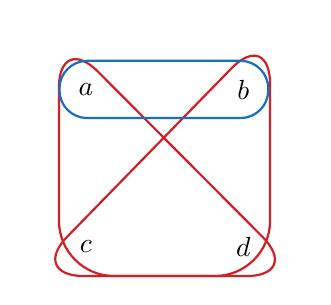
\begin{tikzpicture}
			\node[] at (0,0) (a) {$a$};
			\node[] at (2, 0) (b) {$b$};
			\node[] at (0, -2) (c) {$c$};
			\node[] at (2, -2) (d) {$d$};
			
			\node[fit=(a) (c) (d)] (acd) {};
			\draw[rounded corners=20pt, thick, rwth-red] ($(acd.north west)+(0,0.4)$) -- (acd.south west) -- ($(acd.south east)+(0.4,0)$) -- cycle;
			
			\node[fit=(b) (c) (d)] (bcd) {};
			\draw[rounded corners=20pt, thick, rwth-red] ($(bcd.north east)+(0,0.4)$) -- (bcd.south east) -- ($(bcd.south west)+(-0.4, 0)$) -- cycle;
			
			\node[draw, rounded corners=10pt, thick, rwth-blue, fit=(a) (b)] {};
		\end{tikzpicture}
	}
	\hspace*{\fill}
	\subcaptionbox{The binary relational structure $\mathcal{G}_{\mathfrak A}$, where the blue circle represents $U_R$ and the red rectangles represent $U_T$. \label{fig:transformedMultigraph}}[0.49\textwidth]{
		\centering
		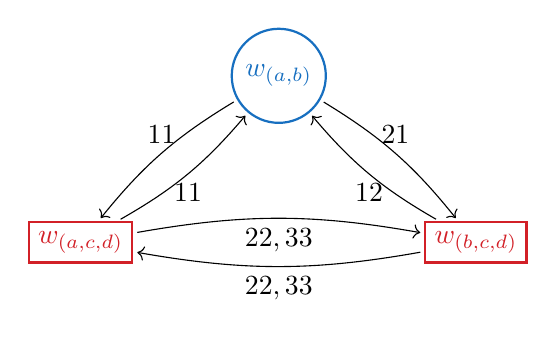
\begin{tikzpicture}[node distance=2cm]
			\node[draw, circle, thick, rwth-blue] (ab) {$w_{(a,b)}$};
			\node[draw, thick, rwth-red, below left=of ab] (acd) {$w_{(a,c,d)}$};
			\node[draw, thick, rwth-red, below right=of ab] (bcd) {$w_{(b,c,d)}$};
			
			\draw
			(ab) edge[shorten >=0.05cm, shorten <=0.05cm, ->, above, bend right=10] node {$11$} (acd)
			(acd) edge[shorten >=0.05cm, shorten <=0.05cm, ->, below, bend right=10] node {$11$} (ab)
			
			(ab) edge[shorten >=0.05cm, shorten <=0.05cm, ->, above, bend left=10] node {$21$} (bcd)
			(bcd) edge[shorten >=0.05cm, shorten <=0.05cm, ->, below, bend left=10] node {$12$} (ab)
			
			(acd) edge[shorten >=0.05cm, shorten <=0.05cm, ->, below, bend left=10] node {$22,33$} (bcd)
			(bcd) edge[shorten >=0.05cm, shorten <=0.05cm, ->, below, bend left=10] node {$22,33$} (acd);
		\end{tikzpicture}
	}
	\caption{A relational structure $\mathfrak A$ of signature $\sigma=\{R/2, T/3\}$ and the binary relational structure $\mathcal{G}_{\mathfrak{A}}$ that encodes it.}
\end{figure}

We now want to apply RCR on $\mathfrak A$ and then classical CR on $\mathcal{G}_{\mathfrak A}$.
By this we will see that both algorithms generate the same partition of elements.
By the definition, it is obvious that $\rho_0((a,b))=(\{R\},\{(1,1),(2,2)\})$ and $\rho_0((a,c,d))=\rho_0((b,c,d))=(\{T\}, \{(1,1),(2,2),(3,3)\})$.
Thus $(a,b)$ already has a different colour from the other two tuples.
In the next step $(a,c,d)$ and $(b,c,d)$ will also receive different colours.
Concretely,
\begin{align*}
	\rho_1((a,c,d))=(\rho_0((a,c,d)), \leftmultiset
		&(\{(1,1)\}, \rho_0((a,b))), \\
		&(\{(2,2),(3,3)\}, \rho_0((b,c,d))), \\
		&(\{(1,1),(2,2),(3,3)\}, \rho_0((a,c,d)))
	\rightmultiset)
\end{align*}
and
\begin{align*}
	\rho_1((b,c,d))=(\rho_0((b,c,d)), \leftmultiset 
		&(\{(1,2)\}, \rho_0((a,b))), \\
		&(\{(2,2),(3,3)\}, \rho_0((a,c,d))), \\
		&(\{(1,1),(2,2),(3,3)\}, \rho_0((b,c,d)))
	\rightmultiset).
\end{align*}
It can thus be seen that $\rho_1((a,c,d))\neq \rho_1((b,c,d))$.
The algorithm has now found a stable colouring, as all elements have a distinct colour.

We will now get the same results when applying classical Colour Refinement to $\mathcal{G}_{\mathfrak A}$.
Similarly to RCR, we have $\gamma_0(w_{(a,b)})=(\{U_R\}, \{E_{1,1},E_{2,2}\})$ and $\gamma_0(w_{(a,c,d)})=\gamma_0(w_{(b,c,d)})=(\{U_T\}, \{E_{1,1},E_{2,2},E_{3,3}\})$.
As before, $w_{(a,c,d)}$ and $w_{(b,c,d)}$ share the initial colour, while $w_{(a,b)}$ has a distinct one.
For the second round we now get 
\begin{align*}
	\gamma_1(w_{(a,c,d)})=(\gamma_0(w_{(a,c,d)}), \leftmultiset
		&(\{E_{1,1}^+,E_{1,1}^-\}, \gamma_0(w_{(a,b)})), \\
		&(\{E_{2,2}^+,E_{3,3}^+, E_{2,2}^-, E_{3,3}^-\}, \gamma_0(w_{(b,c,d)})), \\
		&(\{E_{1,1}^+,E_{2,2}^+,E_{3,3}^+,E_{1,1}^-,E_{2,2}^-,E_{3,3}^-\}, \gamma_0(w_{(a,c,d)}))
	\rightmultiset)
\end{align*}
and
\begin{align*}
	\gamma_1(w_{(b,c,d)})=(\gamma_0(w_{(b,c,d)}), \leftmultiset
	&(\{E_{1,2}^+,E_{2,1}^-\}, \gamma_0(w_{(a,b)})), \\
	&(\{E_{2,2}^+,E_{3,3}^+, E_{2,2}^-, E_{3,3}^-\}, \gamma_0(w_{(a,c,d)})), \\
	&(\{E_{1,1}^+,E_{2,2}^+,E_{3,3}^+,E_{1,1}^-,E_{2,2}^-,E_{3,3}^-\}, \gamma_0(w_{(b,c,d)}))
	\rightmultiset).
\end{align*}
Again, $\gamma_1(w_{(a,c,d)})\neq \gamma_1(w_{(b,c,d)})$ and a stable colouring has been found.
We see that both procedures act equivalently, which is what was proved by Scheidt and Schweikardt.

Let us now look at an example where RCR distinguishes two structures.
For this, consider the $\sigma$-structure $\mathfrak B=(B, R^{\mathfrak B}, T^{\mathfrak B})$ with $B=(a',b',c',d')$, $R^{\mathfrak B}=\{(c',d')\}$ and $T^{\mathfrak B}=\{(a',c',d'),(b',c',d')\}$, which can be seen in Figure \ref{fig:distinguishedByRCR}.
\begin{figure}
	\centering
	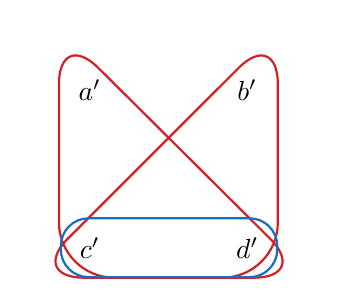
\begin{tikzpicture}
		\node[] at (0,0) (a) {$a'$};
		\node[] at (2, 0) (b) {$b'$};
		\node[] at (0, -2) (c) {$c'$};
		\node[] at (2, -2) (d) {$d'$};
		
		\node[fit=(a) (c) (d)] (acd) {};
		\draw[rounded corners=20pt, thick, rwth-red] ($(acd.north west)+(0,0.4)$) -- (acd.south west) -- ($(acd.south east)+(0.4,0)$) -- cycle;
		
		\node[fit=(b) (c) (d)] (bcd) {};
		\draw[rounded corners=20pt, thick, rwth-red] ($(bcd.north east)+(0,0.4)$) -- (bcd.south east) -- ($(bcd.south west)+(-0.4, 0)$) -- cycle;
		
		\node[draw, rounded corners=10pt, thick, rwth-blue, fit=(c) (d)] {};
	\end{tikzpicture}
	\caption{The $\sigma$-structure $\mathfrak B$ that gets distinguished by RCR from $\mathfrak A$.}
	\label{fig:distinguishedByRCR}
\end{figure}
It can easily be seen that every colour appears exactly as often in the colouring of the tuples of $\mathfrak A$ as of $\mathfrak B$.
Thus $\RCR$ cannot distinguish the structures in round $0$.
However, the colour $\gamma_1((a,c,d))\in \operatorname{RC}_1(\mathfrak A)$ cannot appear in the colouring of $\mathfrak B$.
This is because for all triples $(x,y,z)\in T^{\mathfrak B}$, there does not exist a pair $(x',y')\in R^{\mathfrak B}$, such that $x=x'$.
Therefore $\operatorname{mult}_{\mathfrak A}(\gamma_1((a,c,d)))=1\neq 0 = \operatorname{mult}_{\mathfrak B}(\gamma_1((a,c,d)))$ and RCR distinguishes $\mathfrak A$ and $\mathfrak B$ in round $1$.

In their paper, Scheidt and Schweikardt consider a larger example, which is an extension of the classical non-distinguishable example for Colour Refinement.
They use a signature with a binary relation and a relation of arity $6$.
The example is then comprised of the structure $\mathfrak A_1$ with one $6$-cycle and the structure $\mathfrak A_2$ with two $3$-cycles.
Without the $6$-ary relation the structure would be a regular graph and therefore could not be distinguished by Colour Refinement.
Because of that, the $6$-ary relation includes one tuple, containing all $6$ elements.
With this change, the structures can be distinguished by $\RCR$, which is discussed in \cite{scheidt2025ColorRefinement}.

Furthermore, Scheidt and Schweikardt investigate other, seemingly simpler, possible variants of Colour Refinement which use the Gaifman-Graph and Incidence-Graph of a relational structure.
However, these variants are not able to distinguish $\mathfrak A_1$ and $\mathfrak A_2$, which is why they are disregarded in favour of $\RCR$.

\subsection{Logical Characterisation of RCR}

Classical Colour Refinement gets characterised by counting logic with up to two variables, also called $\C{2}$.
This means that two graphs $G$ and $H$ get distinguished by Colour Refinement if, and only if, there is a sentence $\phi\in \C{2}$, such that $G\models \phi$ and $H\not\models \phi$ \cite{cai1992OptimalLower, immerman1990DescribingGraphs}.
Similarly, Relational Colour Refinement is characterised by the guarded fragment of counting logic, in short $\GFC$.
This logic restricts first-order logic with counting quantifiers in the same way, as the guarded fragment of first-order logic $\mathsf{GF}$ restricts $\mathsf{FO}$.
An investigation of this notion of guards can be found in \cite{gradel1999RestrainingPower}.
The guarded fragment drops the bound on the number of variables, but adds the restriction that quantifiers need be relativised by an atomic formula.

\begin{definition}[The guarded fragment of counting logic]
	\label{def:GFC}
	For a relational signature $\sigma$, we define the class $\GFC$ over $\sigma$ and for a formula $\phi\in \GFC$ the set of variables $\free{\phi}$ inductively, using the following rules:
	\begin{enumerate}
		\item Let $R\in\sigma$ with $\ell=\operatorname{ar}(R)$ and let $x_1,\dots,x_\ell$ be variables. Then $R(x_1,\dots,x_\ell)\in \GFC$ and $\free{R(x_1,\dots,x_\ell)}=\{x_1,\dots,x_\ell\}$.
		\item Let $x$ and $y$ be two variables. 
		Then $x=y\in\GFC$ and $\free{x=y}=\{x,y\}$.
		\item Let $\phi\in\GFC$.
		Then $(\neg\phi)\in\GFC$ and $\free{(\neg\phi)}=\free{\phi}$.
		\item Let $\phi,\psi,\in\GFC$. 
		Then $(\phi\land\psi)\in\GFC$ and $\free{(\phi\land\psi)}=\free{\phi}\cup\free{\psi}$.
		\item For a formula built using Rule \emph{1.} or \emph{2.} $\Delta$ and a $\phi\in\GFC$, we call $\Delta$ a guard for $\phi$, if $\free{\Delta}\supseteq\free{\phi}$.
		Let $\Delta,\phi\in \GFC$, where $\Delta$ is a guard for $\phi$, let $\mathbf v$ be a tuple of variables with $\set(\mathbf v)\subseteq \free{\Delta}$ and let $n\in \mathbb N_{\geq 1}$. 
		Then $\exists^{\geq n}\mathbf v . (\Delta \land \phi)\in \GFC$ and $\free{\exists^{\geq n}\mathbf v.(\Delta\land\phi)}=\free{\Delta}\setminus \set(\mathbf v)$.
	\end{enumerate}
	Formulae that are built using Rules \emph{1.} and \emph{2.} are called atomic formulae, we omit parenthesises in the usual way and use $\exists^{=n}\mathbf v.(\Delta\land\phi)$ as shorthand notation for $\exists^{\geq n}\mathbf v.(\Delta\land\phi)\land \neg\exists^{\geq n+1}\mathbf v.(\Delta\land\phi)$.
	
	The semantics of this logic are analogous to classical counting logic, see for example \cite{cai1992OptimalLower}, and also are concretely defined in \cite{scheidt2025ColorRefinement}.
\end{definition}
When comparing $\GFC$ with the logic $\mathsf{GC}^1$, see \cite{scheidt2023CountingHomomorphisms}, we notice that they seem very similar.
A guard in $\GFC$ uses only one edge, since atomic formulae are either equalities or relations.
This is similar to the one available edge variable in $\mathsf{GC}^1$, over which a guard is defined.

Using a pebble game for $\GFC$, called the Guarded-Game, Scheidt and Schweikardt proved the following theorem:
\begin{theorem}[Theorem B from \cite{scheidt2025ColorRefinement}]
	Let $\sigma$ be a relational signature and let $\mathfrak A$ and $\mathfrak B$ be $\sigma$-structures.
	Then the three following statements are equivalent:
	\begin{enumerate}
		\item Relational Colour Refinement distinguishes $\mathfrak A$ and $\mathfrak B$.
		\item There exists a sentence $\phi\in \GFC$ such that $\mathfrak A\models \phi$ and $\mathfrak B\not\models\phi$.
		\item Spoiler wins the Guarded-Game on $\mathfrak A$ and $\mathfrak B$.
	\end{enumerate}
\end{theorem}
Let us again consider the structures from Figures \ref{fig:verySimpleRelStruc} and \ref{fig:distinguishedByRCR}.
In the preceding section we used the colour $\rho_1((a,c,d))$ to distinguish $\mathfrak A$ and $\mathfrak B$, as it does not appear in the colouring of $\mathfrak B$.
More precisely, there does not exist a tuple of length $3$ in $\mathfrak B$, which is in the relation $T$ and its first element is in the relation $R$ with another element.
This can be formalised using the formula
$$\phi_1\coloneqq\exists^{\geq 1}(x,y,z).\left(T(x,y,z)\land \exists^{\geq 1} (y).\left( R(x,y)\right)\right).$$
It is easy to see that $\mathfrak A\models \phi_1$ and $\mathfrak B\not\models \phi_1$.

\subsection{Characterising RCR by Homomorphism Counting}

Another way to characterise classical CR is to count homomorphisms from trees.
Due to \cite{dvorak2010RecognizingGraphsa} and \cite{dell2018LovaszMeets} it is known that Colour Refinement distinguishes two graphs $G$ and $H$ if, and only if, there is a tree $T$, such that $\hom(T,G)\neq\hom(T,H)$.
Again, there is an analogous characterisation for Relational Colour Refinement.
One obstacle in defining such a characterisation is finding a class that generalises trees for relational structures.
As a tree is a connected, acyclic graph, we have to find a fitting notion of acyclicity for relational structures.
It can be seen, for example in \cite{brault-baron2014HypergraphAcyclicity}, that there are multiple such definitions for hypergraphs, which can be applied to relational structures as well.
When considering the results from \cite{scheidt2023CountingHomomorphisms} and that $\mathsf{GC}^1$ seems very similar to $\GFC$, it appears that hypergraphs of generalised hypertree width of $1$, or equivalently $\alpha$-acyclic hypergraphs, may be a possible candidate.
This is in fact the case.
Let us therefore define $\alpha$-acyclic structures, which will just be called acyclic structures in the following.

\begin{definition}[Acyclic structures]
	\label{def:alphaAcyclic}
	Let $\sigma$ be a relational signature and let $\mathfrak C$ be a $\sigma$-structure.
	A join-tree $J$ for $\mathfrak C$ is a tree with a vertex for every tuple in $\mathfrak C$, thus $V(J)=\mathbf C$, which fulfils the join-tree-property:
	For any $c\in C$, the set $\{\mathbf c \in V(J) : c\in \set(\mathbf c)\}$ induces a connected subgraph of $J$.
	This induced subgraph is also a tree and will be denoted as $J_c$.
	Finally, we call a structure acyclic, if it has a join-tree.
\end{definition}
There are multiple equivalent characterisations for this notion of acyclicity which can be found in \cite{brault-baron2014HypergraphAcyclicity}.
Recall the definition for homomorphisms between structures and the definitions of $\Hom$ and $\hom$.
This then leads us to another main result from \cite{scheidt2025ColorRefinement}.

\begin{theorem}[Theorem A from \cite{scheidt2025ColorRefinement}]
	Let $\sigma$ be a relational signature and let $\mathfrak A$ and $\mathfrak B$ be $\sigma$-structures.
	Then the two following statements are equivalent:
	\begin{enumerate}
		\item Relational Colour Refinement distinguishes $\mathfrak A$ and $\mathfrak B$.
		\item There exists an acyclic $\sigma$-structure $\mathfrak C$, such that $\hom(\mathfrak C,\mathfrak A)\neq\hom(\mathfrak C,\mathfrak B)$.
	\end{enumerate}
\end{theorem}

We again want to consider the structures from Figures \ref{fig:verySimpleRelStruc} and \ref{fig:distinguishedByRCR} for a simple example.
The structure $\mathfrak B$ is acyclic.
This can be seen from its join tree depicted in Figure \ref{fig:distinguishedJoinTree}.
\begin{figure}
	\centering
	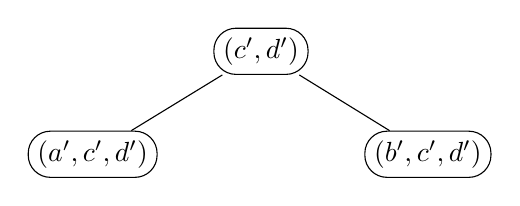
\begin{tikzpicture}[node distance=1cm]
		\node[draw, rounded corners=8pt] (cd) {$(c',d')$};
		\node[draw, rounded corners=8pt, below left=of cd] (acd) {$(a',c',d')$};
		\node[draw, rounded corners=8pt, below right=of cd] (bcd) {$(b',c',d')$};
		
		\draw
		(cd) edge[-] (acd)
		(cd) edge[-] (bcd);
	\end{tikzpicture}
	\caption{A join-tree for the structure $\mathfrak B$ from Figure \ref{fig:distinguishedByRCR}}
	\label{fig:distinguishedJoinTree}
\end{figure}
Now consider the homomorphisms from $\mathfrak B$.
The identity is always a homomorphism, therefore $\hom(\mathfrak B, \mathfrak B)\geq 1$.
However, a homomorphism from $\mathfrak B$ to $\mathfrak A$ cannot exist.
Consider $(c',d')\in R^{\mathfrak B}$ and that $(a,b)$ is the only tuple in $R^{\mathfrak A}$. 
We therefore would have to map $c'$ to $a$ and $d'$ to $b$.
But now consider the tuple $(a',c',d')\in T^{\mathfrak B}$ and let $x$ be the element that $a'$ gets mapped to.
Then $(x,a,b)$ must be in $T^{\mathfrak A}$.
But there is no such tuple in $\mathfrak A$, independently of $x$.
Therefore there cannot exist a homomorphism from $\mathfrak B$ to $\mathfrak A$, thus $\hom(\mathfrak B, \mathfrak A)=0\neq \hom(\mathfrak B, \mathfrak B)$ and $\mathfrak B$ is an acyclic structure that distinguishes $\mathfrak B$ and $\mathfrak A$ by homomorphism counts.
 


\section{Relational Colour Refinement for structures with functions}
\label{sec:RelationalColourRefinemetForStructuresWithFunctions}

\subsection{Naive Encoding of functions}
\label{Sec::NaiveEncodingOfFunctions}

A simple way to apply relational colour refinement to non-relational structures is, to encode the functions as relations.
Formally we transform a signature $\sigma$ that includes function symbols to a new signature $\sigma'$: 
For every relation symbol $R\in \sigma$, we introduce a relation symbol $R\in \sigma'$ with the same arity and for every function symbol $f\in\sigma$ with arity $k$, we introduce a relational symbol $R_f\in\sigma'$ of arity $k+1$.

Semantically, a structure $\mathfrak A$ of signature $\sigma$ can then be encoded as a structure $\mathfrak A'$ of signature $\sigma'$ and with the same universe as $\mathfrak A$. 
For every relational symbol $R\in\sigma$ we set $R^{\mathfrak A'}\coloneqq R^{\mathfrak A}$ and for every function symbol $f\in\sigma$ of arity $k$ there exists a relation symbol $R_f\in\sigma'$ and we set $R_f^{\mathfrak A}\coloneqq \{\mathbf xy : f^{\mathfrak A}(\mathbf x)=y\}$ where $\mathbf x$ is a tuple of arity $k$.

This procedure encodes a non-relational structure as a relational one, on which Relational Colour Refinement can now be performed.
As such we say, that the Naive Relational Colour Refinement (nRCR) distinguishes two structures $\mathfrak A$ and $\mathfrak B$ if, and only if, RCR distinguishes their naive encodings $\mathfrak A'$ and $\mathfrak B'$.
However, this results in a very weak logical characterisation, that does not allow nesting of terms, namely the nesting-free-fragment of $\GFC$.

\begin{definition}[$\mathsf{nfGF}(\mathsf C)$]
	Consider the definition of $\GFC$ given in \ref{}.
	We obtain the nesting-free fragment, by allowing $f(\mathbf x)=y$ as a further atomic formula.
	Concretely, the only allowed atomic formulae are of the form $R(x_1,\dots,x_\ell)$, $x=y$ and $f(x_1,\dots,x_\ell)=y$, where $f$ has arity $\ell$, $\free{f(x_1,\dots,x_\ell)=y}=\{x_1,\dots,x_\ell\}$ and $\gd{f(\mathbf x)=y}=0$.
	
	The remaining definitions stay the same.
\end{definition}

\begin{theorem}
	\label{thm:ThmA}
	The two following statements are equivalent:
	\begin{enumerate}
		\item nRCR distinguishes $\mathfrak A$ and $\mathfrak B$.
		\item There exists a sentence $\phi\in \mathsf{nfGF}(\mathsf C)$ such that $\mathfrak A\models \phi$ and $\mathfrak B\not\models \phi$.
	\end{enumerate}
\end{theorem}
\begin{proof}
	1. $\Rightarrow$ 2.:
	By definition, $\mathfrak A$ and $\mathfrak B$ are distinguished by nRCR if, and only if, $\mathfrak A'$ and $\mathfrak B'$ are distinguished by RCR.
	Using the result of \cite{scheidt2025ColorRefinement}, we obtain a sentence $\varphi'\in\GFC$ that distinguishes the encoded structures.
	Via a structural induction on the formula, we can now translate $\varphi'$ into a formula $\phi\in \mathsf{nfGF}(\mathsf C)$
	This can be achieved by replacing formulae $R_f(x_1,\dots,x_\ell,y)$ by $f(x_1,\dots,x_\ell)=y$ for function symbols $f\in\sigma$ and letting everything else stay the same.
	
	2. $\Rightarrow$ 1.:
	When considering $\mathsf{nfGF}(\mathsf C)$, one can find that the transformation done at the end of the first direction can be applied in reverse.
	This then leads to a distinguishing sentence in $\GFC$ and with \cite{scheidt2025ColorRefinement} to a distinguishing colouring of the encoded structures, which by definition is a distinguishing colouring for the structures themselves.
\end{proof}

While the above theorem results in a nice characterisation of the naive encoding, the nesting of terms is often very desired when using functions.
However, it can be shown that nesting is too powerful for the naive encoding.

Consider the two structures $\mathfrak A$ and $\mathfrak B$ of signature $\sigma=\{f/1\}$ which can be seen in \cref{NaiveEncodingCounterexample}.
Formally they are defined as $\mathfrak A=(A,f^{\mathfrak A})$ and $\mathfrak B = (B, f^{\mathfrak B})$ where

\begin{alignat*}{4}
	A=&\{a_1,a_2,a_3,a_4,a_5,a_6\}, &&  && B=&&\{b_1,b_2,b_3,b_4,b_5,b_6\},\\
	f^{\mathfrak A}=&\{a_1\mapsto a_2, a_2\mapsto a_3, a_3 \mapsto a_1, && \qquad \text{and} \qquad && f^{\mathfrak B}=&&\{b_1 \mapsto b_2, b_2 \mapsto b_3, b_3 \mapsto b_4, \\
	&\phantom{\{} a_4\mapsto a_5, a_5\mapsto a_6, a_6\mapsto a_4 \} &&  && && \phantom{\{} b_4 \mapsto b_5, b_5 \mapsto b_6, b_6 \mapsto b_1\}
\end{alignat*}

\begin{figure}
	\centering
	\begin{multicols}{2}
		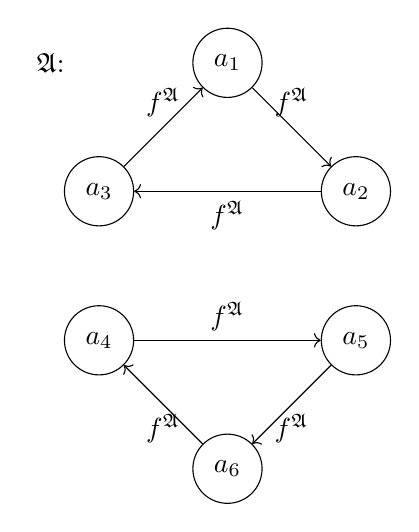
\begin{tikzpicture}
			\node[state] (a1) {$a_1$};
			\node[left=of a1, xshift=-0.5cm] (label) {$\mathfrak A$:};
			\node[state, below left=of a1] (a3) {$a_3$};
			\node[state, below right=of a1] (a2) {$a_2$};
			\node[state, below =of a3] (a4) {$a_4$};
			\node[state, below =of a2] (a5) {$a_5$};
			\node[state, below left=of a5] (a6) {$a_6$};
			\draw 
			(a1) edge[->, above] node{$f^{\mathfrak A}$} (a2)
			(a2) edge[->, below] node{$f^{\mathfrak A}$} (a3)
			(a3) edge[->, above] node{$f^{\mathfrak A}$} (a1)
			(a4) edge[->, above] node{$f^{\mathfrak A}$} (a5)
			(a5) edge[->, below] node{$f^{\mathfrak A}$} (a6)
			(a6) edge[->, below] node{$f^{\mathfrak A}$} (a4);
		\end{tikzpicture}
		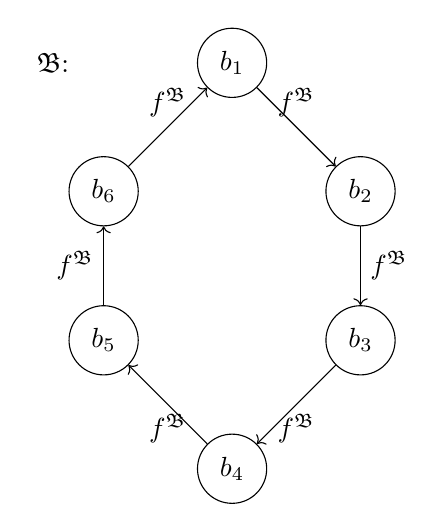
\begin{tikzpicture}
			\node[state] (b1) {$b_1$};
			\node[left=of b1, xshift=-0.5cm] (label) {$\mathfrak B$:};
			\node[state, below left=of b1] (b6) {$b_6$};
			\node[state, below right=of b1] (b2) {$b_2$};
			\node[state, below =of b2] (b3) {$b_3$};
			\node[state, below =of b6] (b5) {$b_5$};
			\node[state, below left=of b3] (b4) {$b_4$};
			\draw 
			(b1) edge[->, above] node{$f^{\mathfrak B}$} (b2)
			(b2) edge[->, right] node{$f^{\mathfrak B}$} (b3)
			(b3) edge[->, below] node{$f^{\mathfrak B}$} (b4)
			(b4) edge[->, below] node{$f^{\mathfrak B}$} (b5)
			(b5) edge[->, left] node{$f^{\mathfrak B}$} (b6)
			(b6) edge[->, above] node{$f^{\mathfrak B}$} (b1);
		\end{tikzpicture}
	\end{multicols}
	
	\caption{Two $\sigma$-structures $\mathfrak A$ and $\mathfrak B$ which can be distinguished by $\GFC$, but not by $\operatorname{nRCR}$.}
	\label{NaiveEncodingCounterexample}
\end{figure}

Consider the formula $\phi=\exists^{\geq 1} x.(f(f(f(x)))=x)$ which utilizes term nesting to find a cycle of length three.
It is obvious that $\mathfrak A \models \phi$ and $\mathfrak B\not\models \phi$.
However, when encoding the two structures with the naive method described above, one finds that nRCR cannot distinguish them.
Therefore, term nesting is too powerful for the naive encoding.

A method that allows for the nesting of terms will be described in the following section.


\subsection{Using the transitive expansion} 
\label{sec:TransitiveExpansion}

As a first remark we note that we only consider unary functions in this section.
The key idea will be, to encode a function $f$ as a family of relations, which then can capture the notion of nesting function applications.
However, a bound on the alternation of different function symbols is necessary to ensure that the expanded signature is still finite, thus we will fixate a maximal alternation depth when discussing our new variant of $\RCR$.
Let us now concretely define, how we expand the signature.

\begin{definition}[Transitive Expansion]
	Let $\sigma\coloneqq \sigma_{\operatorname{Rel}} \operatorname{\dot{\cup}} \sigma_{\operatorname{Func}}$ be a signature with relation symbols $\sigma_{\operatorname{Rel}}$ and unary function symbols $\sigma_{\operatorname{Func}}$ and let $\mathfrak A$ be a structure of signature $\sigma$ with $\Vert \mathfrak A \Vert=n$.
	For readability, we define the family of sets of alternations of function applications $\operatorname{Alters}_n^0(\sigma)\coloneqq\{\operatorname{id}\}$ and
	\begin{align*}
		\operatorname{Alters}^k_{n}(\sigma)\coloneqq \operatorname{Alters}^{k-1}_{n}(\sigma)\cup\{f_1^{m_1}f_2^{m_2}\dots f_k^{m_k} : & f_1f_2\dots f_k\in (\sigma_{\operatorname{Func}})^k \\ 
		& \land 0 < m_i \leq n \text{ for } i \in [k] \\ 
		& \land \forall i\in\{1,\dots,k-1\} . f_{i-1}\neq f_i \neq f_{i+1}\}.
	\end{align*}
	We will now fixate an arbitrary $k\in\mathbb N$ which will be our bound on the alternation depth and will define a new signature $\widetilde{\sigma}$ as well as a structure $\widetilde{\mathfrak A}$ of said signature, which will be the transitive expansion with alternation depth $k$ of $\mathfrak{A}$.
	For $k\in\mathbb N$, $\alpha,\beta,\alpha_1,\dots,\alpha_\ell\in \operatorname{Alters}^k_n(\sigma)$ and a $R\in \sigma_{\operatorname{Rel}}$ with arity $\ell$, we define the binary relation
	$$\operatorname{Eq}_{\alpha,\beta}^{\widetilde{\mathfrak A}}\coloneqq \{(a,b) : \alpha^{\mathfrak A}(a)=\beta^{\mathfrak A}(b)\},$$
	and the relation of arity $\ell$
	$$R_{\alpha_1,\dots,\alpha_\ell}^{\widetilde{\mathfrak A}} \coloneqq \{(a_1,\dots,a_\ell) : (\alpha_1^{\mathfrak A}(a_1),\dots,\alpha_\ell^{\mathfrak A}(a_\ell))\in R^{\mathfrak A}\}.$$
	We now define the transitive expansion with alternation depth $k$ signature $\widetilde{\sigma}$, where 
	\begin{align*}
		\widetilde{\sigma}\coloneqq & \{\operatorname{Eq}_{\alpha,\beta}: \alpha,\beta\in\operatorname{Alters}^k_n(\sigma)\}, \\
		& \operatorname{\dot{\cup}} \{R_{\alpha_1,\dots,\alpha_\ell} : R\in \sigma_{\operatorname{Rel}},\operatorname{ar}(R)=\ell \text{ and } \alpha\in \operatorname{Alters}^k_n(\sigma)\}.
	\end{align*}
\end{definition}

Since the following definitions will depend on this construction, let us consider an example.
We define the signature $\sigma=\{R,f,g\}$ where $R$ is a unary relation symbol and $f$ and $g$ are unary function symbols.
Now consider a $\sigma$ structure $\mathfrak A=(A,\sigma)$ with $A=\{a,b\}$, $R^{\mathfrak A}=\{a\}$, $f^{\mathfrak A}=\{a\mapsto b, b\mapsto a\}$ and $g^{\mathfrak A}=\{a\mapsto a, b\mapsto b\}$.
A graphical representation of $\mathfrak A$ can be found in \cref{TransitiveExpansionExample}.
For the sake of simplicity we will define the transitive expansion with alternation depth $1$ and because $\Vert\mathfrak A\Vert=2$ we will use $\operatorname{Alters}^1_2(\sigma)$ to do so.
We see that $\operatorname{Alters}^1_2(\sigma)=\{\operatorname{id}, f,f^2,g,g^2\}$ and as such 
$$\widetilde{\sigma}=\{R_{\operatorname{id}}, R_{f}, R_{f^2}, R_g, R_{g^2}, \operatorname{Eq}_{\operatorname{id},\operatorname{id}}, \operatorname{Eq}_{\operatorname{id},f}, \operatorname{Eq}_{\operatorname{id}, f^2}, \dots, \operatorname{Eq}_{g^2, g^2}\}.$$
Because of the relatively large size of $\widetilde{\sigma}$, we will only give the formal definitions for a few relations, while the rest of the relations in $\widetilde{\mathfrak A}$ can be seen in \cref{TransitiveExpansionExample}.
We find that $R^{\widetilde{\mathfrak A}}_{\operatorname{id}}=R^{\widetilde{\mathfrak A}}_{f^2}=R^{\widetilde{\mathfrak A}}_g=R^{\widetilde{\mathfrak A}}_{g^2}=\{a\}$ and that $R^{\widetilde{\mathfrak A}}_f=\{b\}$.
Additionally, $\operatorname{Eq}^{\widetilde{\mathfrak A}}_{g,\operatorname{id}}=\operatorname{Eq}^{\widetilde{\mathfrak A}}_{g^2,\operatorname{id}}=\{(a,a),(b,b)\}=\operatorname{Eq}^{\widetilde{\mathfrak A}}_{\alpha,\alpha}$ for all $\alpha\in\operatorname{Alters}^1_2(\sigma)$.
To give another example, we have $\operatorname{Eq}^{\widetilde{\mathfrak A}}_{g,f}=\operatorname{Eq}^{\widetilde{\mathfrak A}}_{g^2,f}=\{(a,b),(b,a)\}$.
The definitions of all $\operatorname{Eq}^{\widetilde{\mathfrak A}}_{\alpha,\beta}$ can be found in \cref{TransitiveExpansionExample}.

\begin{figure}[h]
	\centering
	\begin{multicols}{2}
		\begin{tikzpicture}[node distance=3cm]
			\node[state] (a) {$a$};
			\node[state, right=of a] (b) {$b$};
			\node[left=of a1, xshift=2cm] (label) {$\mathfrak A$:};
			\draw 
			(a) edge[->, thick, above, bend left] node{$f$} (b)
			(b) edge[->, thick, below, bend left] node{$f$} (a)
			(a) edge[->, thick, loop left] node{$g$} (a)
			(b) edge[->, thick, loop right] node{$g$} (b);
		\end{tikzpicture}
		\begin{tikzpicture}[node distance=3cm]
			\node[state] (a) {$a$};
			\node[state, right=of a] (b) {$b$};
			\node[left=of a1, xshift=2cm] (label) {$\widetilde{\mathfrak A}$:};
			\draw 
			(a) edge[->, thick, above, bend left, rwth-blue] node{\phantom{$f$}} (b)
			(b) edge[->, thick, below, bend left, rwth-blue] node{} (a)
			(a) edge[->, thick, loop left, rwth-red] node{} (a)
			(b) edge[->, thick, loop right, rwth-red] node{} (b);
		\end{tikzpicture}
	\end{multicols}
	\caption{Graphical description of $\mathfrak A$ and $\widetilde{\mathfrak A}$. The blue transitions represent the relations $\operatorname{Eq}_{\alpha,\beta}$ with $(\alpha,\beta)\in\{(\operatorname{id},f),(f,\operatorname{id}), (f,f^2),(f,g),(f,g^2),(f^2,f),(g,f),(g^2,f)\}$, while the red transitions represent all other binary relations.}
	\label{TransitiveExpansionExample}
\end{figure}

We can now define $\RCR$ for signatures that include unary function symbols.

\begin{definition}[RCR for structures with unary functions]
	Let $\sigma$ be a signature with relation and unary function symbols and let $\mathfrak A$ and $\mathfrak B$ be structures of signature $\sigma$.
	
	We say that $\mathfrak A$ and $\mathfrak B$ are being distinguished by RCR with alternation depth $k$ ($\RCR_k$), if $\Vert\mathfrak A\Vert\neq \Vert \mathfrak B\Vert$ or the transitive expansions with alternation depth $k$, $\widetilde{\mathfrak A}$ and $\widetilde{\mathfrak B}$, are being distinguished by $\RCR$.
\end{definition}

To show that this definition may be sensible, we want to see, whether $\RCR_1$ distinguishes the structures $\mathfrak A$ and $\mathfrak B$ from \cref{NaiveEncodingCounterexample}.
First we compute $\widetilde\sigma$ as $\{\operatorname{Eq}_{f^i,f^j}, \operatorname{Eq}_{f^i,\operatorname{id}}, \operatorname{Eq}_{\operatorname{id},f^j} : 0\leq i,j \leq 6\}\cup\{\operatorname{Eq}_{\operatorname{id},\operatorname{id}}\}$. 
For easier readability, we will only give the definitions for the symbols in $\{\operatorname{Eq}_{f^i,\operatorname{id}} : 0 \leq i \leq n\}$. 
In fact, we find that 
$$\operatorname{Eq}_{f^i,\operatorname{id}}^{\widetilde{\mathfrak A}} = \{(a_j,a_{j+i \mod 3}) : j \in [6]\}$$
and 
$$\operatorname{Eq}_{f^i,\operatorname{id}}^{\widetilde{\mathfrak B}} = \{(a_j,a_{j+i \mod 6}) : j \in [6]\}.$$
By using \cite{scheidt2025ColorRefinement}, we know that $\RCR$ distinguishes $\widetilde{\mathfrak A}$ and $\widetilde{\mathfrak B}$ if, and only if, there is a formula $\widetilde{\phi}\in\GFC$ of signature $\widetilde{\sigma}$ that distinguishes them.
Notice that $\operatorname{Eq}_{f^0,\operatorname{id}}^{\widetilde{\mathfrak A}}=\operatorname{Eq}_{f^3,\operatorname{id}}^{\widetilde{\mathfrak A}}=\operatorname{Eq}_{f^6,\operatorname{id}}^{\widetilde{\mathfrak A}}$, $\operatorname{Eq}_{f^1,\operatorname{id}}^{\widetilde{\mathfrak A}}=\operatorname{Eq}_{f^4,\operatorname{id}}^{\widetilde{\mathfrak A}}$ and $\operatorname{Eq}_{f^2,\operatorname{id}}^{\widetilde{\mathfrak A}}=\operatorname{Eq}_{f^5,\operatorname{id}}^{\widetilde{\mathfrak A}}$, while only $\operatorname{Eq}_{f^0,\operatorname{id}}^{\widetilde{\mathfrak B}}=\operatorname{Eq}_{f^6,\operatorname{id}}^{\widetilde{\mathfrak B}}$.
Therefore the sentence 
$$\exists^{\geq 6}(x,y).\left(\operatorname{Eq}_{f^1,\operatorname{id}}(x,y) \land \operatorname{Eq}_{f^4,\operatorname{id}}(x,y)\right)\in \GFC$$ 
is satisfied by $\widetilde{\mathfrak A}$, but not $\widetilde{\mathfrak B}$.
Furthermore, consider the formula $\phi=\exists^{\geq 1} x.(f(f(f(x)))=x)$ that has been to used to distinguish $\mathfrak A$ and $\mathfrak B$.
We can easily derive another formula $\phi'\in \GFC$ to distinguish the transitive expansions, namely $\phi'=\exists^{\geq 1} x. \operatorname{Eq}_{f^3, \operatorname{id}}(x, x)$.

We see that this procedure distinguishes structures that were not distinguished by nRCR.
In the following, we want to investigate how much stronger this new algorithm is, by finding a logic that characterises it.

\subsubsection{Logical characterisation of $\RCR_k$}

A first idea that may come to mind when looking at the definition of the transitive expansion, is to use the classical notion of atomic formula for guards, fixate a maximal alternation depth for terms and only allow $\Vert \mathfrak{A}\Vert$ applications of the same function symbol on series, that is, only allow $f^m(s(x))$ where $m<\Vert\mathfrak A\Vert$.
However, we prove that we can allow any $f^m(s(x))$, while the bounded alternation depth is still needed.
The reason why this is possible, hinges on the pigeonhole principle.
When considering $f(x)$, $f^2(x)$, $f^3(x)$ and so forth, until $f^m(x)$, where $m>\Vert\mathfrak A\Vert$, there have to be to numbers $i$ and $j$, such that $f^i(x)=f^j(x)$.
Therefore, we can decompose the path into a path to a cycle, the cycle itself, and a last part of that cycle.
To allow the following proofs to be more readable, we first want to define the set of all such valid decompositions.

Let 
\begin{align*}
	\mathcal I(n,m)=\{(k,l,p)\in [n]^3 \quad:\quad & k+p < k+l \leq n \; \land \\
	& k+r\cdot l + p = m \text{ for some } r\in \mathbb N\}.
\end{align*}
This set will represents all the possible ways, to decompose a path into a cycle and the path to and from it.
This means, that the triple $(k,\ell,p)$ will represent a path, that has a beginning part of length $k$, then a cycle of length $\ell$ and a last part that consists of the first $p$ elements of the cycle.
One can see that in a structure $\mathfrak A$ with a unary function $f$ and $n$ elements, any path along of $f$ with length $m>n$ can be decomposed into a triple in the set $\mathcal I(n,m)$.
A graphical description of such a triple $(k,\ell,p)$ can be found in \cref{PathDecompositionPrinciple}.

\begin{figure}[h]
	\centering
	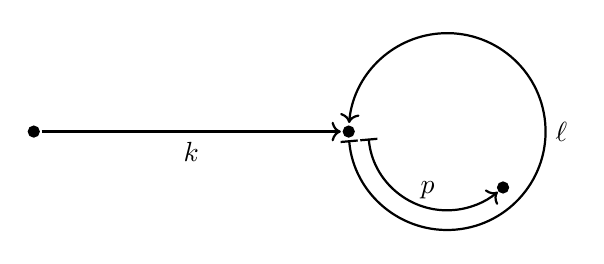
\begin{tikzpicture}
		\filldraw (-2, 0) circle (2pt); % Begin
		\draw[thick, ->] (-1.9, 0) -- node[below] {$k$} (1.9, 0) ;
		\filldraw (2, 0) circle (2pt); % End of k
		\draw[thick, |->] (3.25, 0) ++(-175:1.25) arc (-175:175:1.25);
		\node[xshift=4.7cm] {$\ell$};
		\draw[thick, |->] (3.25, 0) ++(-175:1) arc (-175:-50:1);
		\node[xshift=3cm, yshift=-0.75cm] {$p$};
		\filldraw (3.96, -0.71) circle (2pt);
	\end{tikzpicture}
	
	\caption{A description of how a path can be decomposed into a cycle, the path to it and a last part of it.}
	\label{PathDecompositionPrinciple}
\end{figure}

In the beginning we remarked that we have to fixate an alternation depth.
This bound can be seen in the definition of the transitive expansion and will be used in the logic that will characterise the Colour Refinement algorithm.
Therefore we can only reason about a fragment of $\GFC$, where the terms do not alternate too often.
This is formally stated in the following definition.

\begin{definition}[Alternation bounded $\GFC$]
	The fragment of $\GFC$ with an bounded alternation depth of $k$ ($\GFC_k$) is $\GFC$ with the constraint that for all formulae $\phi\in\GFC_k$ of signature $\sigma$ and every term $t$ that appears in $\phi$, there is an $n\in \mathbb{N}$ and an $\alpha\in \operatorname{Alters}_n^k(\sigma)$ such that $\alpha=t$.
	Atomic formulae are defined as usual, that is, the formulae $R(t_1(x_1),t_2(x_2),\dots,t_n(x_n))$ and $t_1(x_1)=t_2(x_2)$ for terms $t_1,t_2,\dots,t_n$ and variables $x_1,x_2,\dots,x_n$ are atomic formulae.
\end{definition}

With this, we can prove the first result, which allows us to use every $f^m(x)=y$ in a formula.

\begin{lemma}
	Let $\psi(x_1,x_2)\in \GFC_1$ be of the form $f^m(x_1)=x_2$. 
	Then there exists a formula $\theta(x_1,x_2)\in \GFC$ such that for any $\mathfrak A$ with $\Vert \mathfrak A\Vert=n$ it holds
	$$\mathfrak A,a_1,a_2 \models \psi(x_1,x_2) \text{ if, and only if, } \mathfrak A,a_1,a_2 \models \theta(x_1,x_2)$$ 
	and for any $f^{m'}(x)$ that appears in $\theta$ we have $m'\leq n$.
	Furthermore, $\theta(x_1,x_2)$ is of the form $\bigvee \Phi(x_1,x_2)$, and if $\mathfrak A,a_1,a_2\models \theta(x_1,x_2)$, then there is exactly one $\phi(x_1,x_2)\in\Phi$, such that $\mathfrak A,a_1\models \exists^{\geq 1} x_2 . \phi(x_1,x_2)$.
	Additionally, $\theta(x_1,x_2)\in \GFC_1$.
	\label{Simple_fm_to_fk}
\end{lemma}
\begin{proof}
	If $m \leq n$, we let $\theta\coloneqq\psi$ and the claim follows.
	
	Otherwise, we define
	$$\theta(x_1,x_2)\coloneqq \bigvee_{(k,\ell,p)\in \mathcal I(n,m)} \zeta_{(k,\ell,p)}(x_1,x_2)$$
	where
	\begin{align*}
		\zeta_{(k,\ell,p)}(x_1,x_2)\coloneqq & f^{k+p}(x_1)=x_2 \land f^{k}(x_1)=f^{k+\ell}(x_1) \\
		& \land \operatorname{E}^{k,\ell}_{f}(x_1)  \\
		& \land \bigwedge_{\ell'<\ell}f^{k}(x_1)\neq f^{k+\ell'}(x_1)
	\end{align*}
	and for some term $t(x_1)$ we have
	$$\operatorname{E}^{k,\ell}_{f}(t(x_1))=\begin{cases}
		\top & \text{if } k=0 \\
		f^{k-1}(t(x_1))\neq f^{k-1+\ell}(t(x_1)) & \text{otherwise}.
	\end{cases}$$
	Due to the definition of $\mathcal I(n,m)$ it is obvious that only $f^{m'}$ with $m'\leq n$ appears.
	We now proceed to the proof of the equivalence.
	For the purpose of readability, we will write $f_{\mathfrak A}$ instead of $f^{\mathfrak A}$.
	
	We will show that if $\mathfrak A,a_1,a_2 \models \theta(x_1,x_2)$, then $\mathfrak A,a_1,a_2 \models \psi(x_1,x_2)$.
	Let $\mathfrak A,a_1,a_2 \models \theta(x_1,x_2)$. 
	By definition of $\theta$, there are $(k,\ell,p)\in \mathcal I(n,m)$ with $\mathfrak A,a_1,a_2 \models \zeta_{(k,\ell,p)}(x_1,x_2)$.
	In particular $f_{\mathfrak A}^{k}(a_1)=f_{\mathfrak A}^{k+\ell}(a_1)$. It follows that
	$$f_{\mathfrak A}^{k}(a_1)=f_{\mathfrak A}^{k+\ell}(a_1)=f_{\mathfrak A}^{k+2\ell}(a_1)=f_{\mathfrak A}^{k+3\ell}(a_1) = \dots = f_{\mathfrak A}^{k+r\cdot \ell}(a_1)$$
	for all $r\in \mathbb N$. By using the definition of $\mathcal{I}(n,m)$, we get
	$$a_2 =f_{\mathfrak A}^{k+p}(a_1) = f_{\mathfrak A}^{k+r\cdot \ell + p}(a_1)=f_{\mathfrak A}^{m}(a_1).$$
	From this we can deduce $\mathfrak A,a_1,a_2\models \psi(x_1,x_2)$, where $\psi(x_1,x_2)$ has the form $f^{m}(x_1)=x_2$.
	
	Now we prove that if $\mathfrak A,a_1,a_2 \models \psi(x_1,x_2)$, then $\mathfrak A,a_1,a_2 \models \theta(x_1,x_2)$. 
	Let $\mathfrak A,a_1,a_2\models \psi(x_1,x_2)$. By assumption $m>n$ and by the pigeonhole principle there have to be distinct $i$ and $j$ such that $f_{\mathfrak A}^{i}(a_1)=f_{\mathfrak A}^{j}(a_1)$.
	Choose such $i$, $j$ such that they are lexicographically minimal.
	Now choose $k\coloneqq i$, $\ell \coloneqq j-i$ and $p\coloneqq (m-i) \mod (j-i)= (m-i) \mod \ell$.
	Obviously $(k,\ell,p)\in\mathcal I(n,m)$ and what remains to be shown is that $\mathfrak A,a_1,a_2\models \zeta_{(k,\ell,p)}(x_1,x_2)$.
	For that, we consider the parts of the conjunction and show for each one that it is satisfied.
	
	\begin{itemize}
		\item $f^{k+p}(x_1)=x_2$ is satisfied.
		We use the fact that $a= b \mod c \Leftrightarrow b = r\cdot c +a \text{ for some } r\in \mathbb N$.
		Then
		$$f_{\mathfrak A}^{k+p}(a_1)=f_{\mathfrak A}^{i+(m-i)-r\cdot \ell}(a_1)=f_{\mathfrak A}^{i+r\cdot \ell + m -i - r\cdot \ell}(a_1)=f_{\mathfrak A}^{m}(a_1)=a_2.$$
		Therefore $\mathfrak A,a_1,a_2\models f^{k+p}(x_1)=x_2$.
		
		\item $f^{k}(x_1)=f^{k+\ell}(x_1)$ is satisfied.
		Consider that
		$$f_{\mathfrak A}^{k}(a_1)=f_{\mathfrak A}^{i}(a_1)=f_{\mathfrak A}^{j}(a_1)=f_{\mathfrak A}^{j+i-i}(a_1)=f_{\mathfrak A}^{i+j-i}(a_1)=f_{\mathfrak A}^{k+\ell}(a_1).$$
		This leads to $\mathfrak A,a_1,a_2\models f^{k}(x_1)=f^{k+\ell}(x_1)$.
		
		\item $\operatorname{E}^{k,\ell}_f(x_1)$ is satisfied.
		Otherwise $f_{\mathfrak A}^{k-1}(a_1)=f_{\mathfrak A}^{k-1+\ell}(a)$, but then $(k-1,\ell)$ would be lexicographically smaller than $(i,j)$.
		
		\item The same reasoning applies to $\bigwedge_{\ell'<\ell}f^{k}(x_1)\neq f^{k+\ell'}(x_1)$. 
		If it weren't satisfied, there would be a $(i,j')$ with $j'<j$ and $f_{\mathfrak A}^{i}(a_1)=f_{\mathfrak A}^{i+j'}(a_1)$ which would be lexicographically smaller than $(i,j)$.
	\end{itemize}
	
	Thus we have shown that every subformula of the conjunction and therefore the formula is being fulfilled.
	
	Lastly, it remains to prove that if $\theta$ is satisfied, then there is exactly one $(k,\ell,p)\in\mathcal{I}(n,m)$ such that $\exists^{\geq 1}x_2.\zeta_{(k,\ell,p)}(x_1, x_2)$ is fulfilled.
	We prove this by contradiction.
	Assume that $\mathfrak A,a_1,a_2\models \theta(x_1,x_2)$ and that there are $\zeta_{(k,\ell,p)}(x_1,x_2)$ and $\zeta_{(k',\ell',p')}(x_1,x_2)$ with $(k,\ell,p)\neq (k',\ell',p')$, such that $\mathfrak A,a_1\models \exists^{\geq 1}x_2.\zeta_{(k,\ell,p)}(x_1,x_2)$ and $\mathfrak A,a_1\models \exists^{\geq 1}x_2.\zeta_{(k',\ell',p')}(x_1,x_2)$.
	
	We proceed with a case distinction. 
	Let $k=k'$ and $\ell=\ell'$.
	Then there are $r,r'\in\mathbb N$ such that
	$$k+r\cdot \ell + p = k'+r'\cdot \ell' + p'=m.$$
	Thus we can infer that $r\cdot \ell+p = r'\cdot \ell'+p'$.
	By definition of $\mathcal{I}(n,m)$ we know that $p,p'<\ell=\ell'$ and as such 
	$$r\cdot \ell +p,r'\cdot \ell'+p'\in \{r\cdot \ell,r\cdot \ell +1,\dots, r\cdot \ell +(\ell-1)\}$$
	and because $p$ is a non-negative integer, $r=r'$ has to follow and further we get $p=p'$.
	However this would contradict that $(k,\ell,p)\neq (k',\ell',p')$.
	Now assume that $\ell\neq\ell'$ and without loss of generality assume that $\ell<\ell'$.
	But then $\mathfrak A,a_1 \not\models \bigwedge_{\hat{\ell}<\ell'}f^{k'}(x_1)\neq f^{k'+\hat{\ell}}(x_1)$, because 
	$$f^{k'+\ell}_{\mathfrak A}(a_1)=f^{k+\ell}_{\mathfrak A}=f^k_{\mathfrak A}(a_1)=f^{k'}_{\mathfrak A}(a_1)$$
	and $k'+\ell < k'+\ell'$.
	Thus this cannot be the case as well.
	
	Consider that $k\neq k'$ and without loss of generality assume that $k<k'$.
	If $\ell=\ell'$, then by the principle of induction, we get that $f_{\mathfrak A}^k(a_1)=f_{\mathfrak A}^{k+\ell}(a_1)$, $f_{\mathfrak A}^{k+1}(a_1)=f_{\mathfrak A}^{k+1+\ell}(a_1)$ and then $f_{\mathfrak A}^{k'}(a_1)=f_{\mathfrak A}^{k'+\ell'}(a_1)$.
	But this contradicts $\mathfrak A,a_1 \models \operatorname{E}^{k',\ell'}_f(x_1)$.
	If $\ell < \ell'$, then 
	$$f_{\mathfrak A}^{k'}(a_1) =f_{\mathfrak A}^{k+(k'-k)}(a_1)=f_{\mathfrak A}^{k+(k'-k)+\ell}(a_1) = f_{\mathfrak A}^{k'+\ell}(a_1),$$
	but this again contradicts $\mathfrak A,a_1 \models \bigwedge_{\hat{\ell}<\ell'}f^{k'}(x_1)\neq f^{k'+\hat{\ell}}(x_1)$.
	If $\ell'<\ell$, then there exists a $t\in\mathbb N$ such that 
	$$k+t\cdot  \ell < k' \leq k+(t+1)\cdot \ell.$$
	We now define $r\coloneqq k+(t+1)\cdot \ell -k'$ and get $f_{\mathfrak A}^{k'+r}(a_1)=f_{\mathfrak A}^{k'+r+\ell'}$ and by using $f_{\mathfrak A}^{k'+r}(a_1)=f_{\mathfrak A}^{k+(t+1)\cdot \ell}(a_1)=f_{\mathfrak A}^k(a_1)$ it follows that $f_{\mathfrak A}^{k}(a_1)=f_{\mathfrak A}^{k+\ell'}(a_1)$.
	This contradicts $\mathfrak A,a_1 \models \bigwedge_{\hat{\ell}<\ell}f^{k}(x_1)\neq f^{k'+\hat{\ell}}(x_1)$.
	
	One can see that we did not use $x_2$ or $a_2$.
	Therefore its interpretation is irrelevant, which is why we can existentially quantify it in the claim.
	As all possible cases lead to a contradiction, the first assumption cannot be true and we proved the claim.
	
	As we did not use any function symbols other than $f$, $\theta(x_1,x_2)\in \GFC_1$ follows obviously.
\end{proof}

The above proof allows for the translation of a formula $f^m(x)=y$ to a formula $\theta(x,y)$ that is equivalent for structures with $n$ elements.
A natural extension would be, to allow alternation of functions, for example formulae like $g^m(f^{m'}(x))=y$.
This is also possible and will be proved in the following.

\begin{lemma}
	Let $d\in\mathbb d$ and $\psi(x_1,x_2)\in \GFC_d$ be of the form $t(x_1)=x_2$ for a term $t$.
	Then there exists a formula $\theta_{t}(x_1,x_2)\in\GFC_d$, such that for any structure $\mathfrak A$ with $\Vert \mathfrak A \Vert = n$ it holds
	$$\mathfrak A,a_1,a_2 \models \psi(x_1,x_2) \text{ if, and only if, } \mathfrak A,a_1,a_2 \models \vartheta_{t}(x_1,x_2).$$ 
	Furthermore, $\theta_{t}(x_1,x_2)$ is of the form $\bigvee \Phi(x_1,x_2)$ where all $\phi(x_1,x_2)\in\Phi(x_1,x_2)$ are of the form
	$$t'(x_1)=x_2 \land \bigwedge \Psi(x_1)$$ 
	for some term $t'(x_1)$, and for every function symbol $f$ in the signature, there does not appear a term of the form $f^m(s(x))$ where $m > n$.
	Additionally, if $\mathfrak A,a_1,a_2\models \theta_{t}(x_1,x_2)$, then there is exactly one $\phi\in\Phi$, such that $\mathfrak A,a_1\models \exists^{\geq 1}x_2.\phi(x_1,x_2)$.
	\label{TranslationOfArbTerms}
\end{lemma}
\begin{proof}
	We prove this via an induction on the term $t(x_1)$.
	
	\textbf{Base case:}
	If $t(x_1)$ is of the form $f^{m}(x_1)$ for a unary function symbol $f$ and $m\in \mathbb N$, we use the formula constructed in the proof of \cref{Simple_fm_to_fk}.
	It can easily be verified that it is in the correct form and from the same proof we get that if the translated formula is fulfilled, exactly one subformula of the disjunction is satisfied.
	
	\textbf{Inductive step:}
	Assume that $t(x_1)$ is of the form $g^m(s(x_1))$ for a unary function symbol $g$, $m\in\mathbb N$ and term $s$.
	By the induction hypothesis, there is a formula $\theta_{s}(x_1,x_2)\in \GFC_{d-1}$ of the form $\bigvee \Phi_s(x_1,x_2)$ defined above with $\mathfrak A,a_1,a_2 \models s(x_1)=x_2$ if, and only if, $\mathfrak A,a_1,a_2\models \theta_{s}(x_1,x_2)$.
	
	If $m\leq n$, we set $\theta_{t}(x_1,x_2)$ to
	$$\bigvee \Phi'(x_1,x_2),$$
	where $\Phi'(x_1,x_2)\coloneqq\{g^{m}(t'(x_1))=x_2 \land \bigwedge \Psi(x_1) : t'(x_1)=x_2 \land \bigwedge \Psi(x_1)\in \Phi_s(x_1,x_2)\}$.
	
	If $m>n$, then we set $\theta_{t}(x_1,x_2)$ to
	$$\bigvee_{(k,\ell,p)\in \mathcal I(n,m)} \bigvee \Phi'_{(k,\ell,p)}(x_1,x_2),$$
	where 
	\begin{align*}
		\Phi'_{(k,\ell,p)}\coloneqq \{g^{k+p}(t'(x_1))=x_2 &\land g^{k}(t'(x_1))=g^{k+l}(t'(x_1)) \\
		& \land \operatorname{E}^{k,l}_g(t'(x_1)) \land \bigwedge_{\ell'<\ell} g^{k}(t'(x_1))\neq g^{k+\ell'}(t'(x_1)) \\
		& \land \Psi(x_1) : t'(x_1)=x_2 \land \bigwedge \Psi(x_1)\in \Phi_s(x_1,x_2)\}
	\end{align*}
	
	By using the above definitions, we get $\mathfrak A,a_1,a_2\models s(x_1)=x_2$ if, and only if, $\mathfrak A,a_1,a_2\models \phi_s(x_1,x_2)$ for some $\phi_s\in\Phi_s$ where $\phi_s(x_1,x_2)$ is of the form $t'(x_1)=x_2 \land \bigwedge \Psi(x_1)$.
	Therefore
	\begin{equation}
		\mathfrak A, a_1,a_2 \models s(x_1)=x_2 \text{ if, and only if, } \mathfrak A,a_1,a_2 \models t'(x_1)=x_2 \land \bigwedge \Psi(x_1).
		\label{Equivalence_s_and_tPsi}
	\end{equation}
	
	We now prove that 
	$$\mathfrak A, a_1,a_2\models t(x_1)=x_2 \text{ if, and only if, } \mathfrak A,a_1,a_2\models \theta_{t}(x_1,x_2).$$
	Assume $m\leq n$.
	Let $\mathfrak A, a_1,a_2 \models \theta_{t}$.
	Then there is some $\phi(x_1,x_2)$ of the form $g^{m}(t'(x_1))=x_2 \land \bigwedge \Psi(x_1)$ such that $\mathfrak A,a_1,a_2\models \phi(x_1,x_2)$.
	We then get
	\begin{align*}
		\mathfrak A,a_1,a_2 \models & g^{m}(t'(x_1))=x_2 \land \bigwedge \Psi(x_1) \\
		\Leftrightarrow \mathfrak A,a_1,a_2,a_3 \models & g^{m}(x_3)=x_2 \land \bigwedge \Psi(x_1) \land t'(x_1)=x_3 \text{ for some } a_3\in A \\
		\overset{(\ref{Equivalence_s_and_tPsi})}{\Leftrightarrow} \mathfrak A,a_1,a_2,a_3\models & g^{m}(x_3)=x_2 \land s(x_1)=x_3 \text{ for some } a_3\in A \\
		\Leftrightarrow \mathfrak A,a_1,a_2 \models & g^{m}(s(x_1))=x_2.
	\end{align*}
	
	Now let $m>n$.
	Then there is a
	\begin{align*}
		\phi(x_1,x_2)\coloneqq g^{k+p}(t'(x_1))=x_2 &\land g^{k}(t'(x_1))=g^{k+l}(t'(x_1)) \\
		& \land \operatorname{E}^{k,l}_g(t'(x_1)) \land \bigwedge_{\ell'<\ell} g^{k}(t'(x_1))\neq g^{k+\ell'}(t'(x_1)) \\
		& \land \bigwedge \Psi(x_1)
	\end{align*}
	for some $(k,\ell,p)\in\mathcal I(n,m)$ with $\mathfrak A,a_1,a_2\models \phi(x_1,x_2)$.
	And now
	\begin{align*}
		\mathfrak A,a_1,a_2 \models & \phi(x_1,x_2) \\
		\Leftrightarrow A,a_1,a_2,a_3 \models &g^{k+p}(x_3)=x_2 \land g^{k}(x_3)=g^{k+l}(x_3) \\
		& \land \operatorname{E}^{k,l}_g(x_3) \land \bigwedge_{\ell'<\ell} g^{k}(x_3)\neq g^{k+\ell'}(x_3) \\
		& \land \bigwedge\Psi(x_1) \land t'(x_1)=x_3 \text{ for some } a_3\in A \\
		\overset{\cref{Simple_fm_to_fk}}{\Leftrightarrow} \mathfrak A, a_1,a_2,a_3 \models & g^{m}(x_3)=x_2 \land t'(x_1)=x_3 \land \bigwedge\Psi(x_1) \text{ for some } a_3 \in A \\
		\overset{\cref{Equivalence_s_and_tPsi}}{\Leftrightarrow} \mathfrak A,a_1,a_2,a_3 \models & g^{m}(x_3)=x_2\land s(x_1)=x_3 \text{ for some } a_3\in A \\
		\Leftrightarrow \mathfrak A,a_1,a_2 \models & g^{m}(s(x_1))=x_2.
	\end{align*}
	The other direction follows in both cases, as only equivalent steps have been used and it is obvious that the disjunction of a set is being fulfilled, if a formula of the set is satisfied.
	
	Lastly, we show that if $\mathfrak A,a_1,a_2\models \theta_t(x_1,x_2)$, where $\theta_t$ is of the form $\bigvee \Phi$, there is exactly one $\phi\in\Phi$, such that $\mathfrak A,a_1\models \exists^{\geq 1} x_2.\phi(x_1,x_2)$.
	As in the proof of \cref{Simple_fm_to_fk}, we are going to use a proof by contradiction and we will look at the cases where $m\leq n$ and $m> n$ separately.
	If $m\leq n$, assume that $\mathfrak A,a_1,a_2\models \theta_t(x_1,x_2)$ and that there are $\phi_1,\phi_2\in \Phi'(x_1,x_2)$ with $\phi_1\neq \phi_2$, $\mathfrak A,a_1\models \exists^{\geq 1}x_2.\phi_1(x_1,x_2)$ and $\mathfrak A,a_1\models \exists^{\geq 1}x_2.\phi_2(x_1,x_2)$.
	It is easy to see that 
	$$\mathfrak A,a_1,a_2\models g^m(t'_1(x_1))=x_2 \land \bigwedge \Psi_1(x_1) \land g^m(t'_2(x_1))=x_2 \land \bigwedge\Psi_2(x_1)$$
	for some $a_2$, which is equivalent to
	$$\mathfrak A,a_1,a_2,a_3,a_4\models g^m(x_3)=x_2 \land t'_1(x_1)=x_3\land \Psi_1(x_1) \land g^m(x_4)=x_2 \land t'_2(x_1)=x_4 \land \Psi_2(x_1)$$
	when using the correct $a_3$ and $a_4$.
	However, $t'_1(x_1)=x_2\land \Psi_1(x_1), t'_2(x_1)=x_s \land \Psi_2(x_1) \in \Phi_s$ and thus there would be $\psi_1(x_1,x_3/x_2),\psi_2(x_1,x_4/x_2) \in \Phi_s$, such that $\mathfrak A,a_1\models \exists^{\geq 1}x_3. \psi(x_1,x_3)$ and $\mathfrak A,a_1\models \exists^{\geq 1}x_4.\psi(x_1,x_4)$.
	This is a contradiction to the induction hypothesis.
	
	If $m>n$, we again assume that $\mathfrak A,a_1,a_2\models \theta_t(x_1,x_2)$ and that there are $\phi_1(x_1,x_2)\in\Phi'_{(k,\ell,p)}(x_1,x_2)$ and $\phi_2(x_1,x_2)\in\Phi'_{(k',\ell',p')}(x_1,x_2)$ with $\phi_1\neq \phi_2$, $\mathfrak A,a_1\models \exists^{\geq 1}x_2.\phi_1(x_1,x_2)$ and $\mathfrak A,a_1\models \exists^{\geq 1}x_2.\phi_2(x_1,x_2)$.
	By looking at the structure of the formulae as they are defined in this proof and by substituting terms and variables like in the first case, we again find that 
	$$\mathfrak A,a_1,a_3,a_4\models t'_1(x_1)=x_3\land \Psi_1(x_1) \land t'_2(x_1)=x_4 \land \Psi_2(x_1),$$
	where $t'_1(x_1)=x_2\land\bigwedge \Psi_1(x_1), t'_2(x_1)=x_2\land\bigwedge \Psi_2(x_1)\in \Phi_2$.
	By using the same arguments as before, we as well arrive at a contradiction.
	As such, the assumption must be false and we have finished the proof.
\end{proof}

A corollary of the above lemma is that the same statement also holds for an arbitrary relation, in addition to equality.

\begin{lemma}
	Let $d\in\mathbb N$ and $\psi(x_1,\dots,x_m)\coloneqq R(t_1(x_1),\dots,t_m(x_m))\in \GFC_d$ be an atomic formula.
	Then there exists a formula $\theta_\psi\in\GFC_d$, such that for any given structure (of fitting signature) $\mathfrak A$ with $\Vert\mathfrak A \Vert=n$ it holds
	$$\mathfrak A,a_1,\dots,a_m\models \psi(x_1,\dots,x_m) \text{ if, and only if, } \mathfrak A,a_1,\dots,a_m\models \theta_\psi(x_1,\dots,x_m).$$
	Furthermore, $\theta_\psi(x_1,\dots,x_m)$ is of the form $\bigvee \Phi(x_1,\dots,x_m)$ where all $\phi\in\Phi$ are of the form
	$$R(t_1'(x_1),\dots,t_m'(x_m))\land \bigwedge\Psi_1(x_1)\land \dots\land\bigwedge \Psi_m(x_m),$$
	and for every $f^m(s(x))$ that appear in $\theta_\psi$, where $f$ is a unary function symbol and $s$ is a term, $m\leq n$.
	Additionally, if $\mathfrak A,a_1,\dots,a_,\models \theta_\psi(x_1,\dots,x_m)$, then there exists exactly one $\phi(x_1,\dots,x_m)\in\Phi(x_1,\dots,x_m)$, such that $\mathfrak A,a_1,\dots,a_m\models \phi(x_1,\dots,x_m)$.
	\label{TranslationOfArbAtomics}
\end{lemma}
\begin{proof}
	Let $\mathfrak A,a_1,\dots,a_m\models\psi(x_1,\dots,x_m)$.
	This is equivalent to 
	$$\mathfrak A,a_1,\dots,a_m,b_1,\dots,b_m\models R(b_1,\dots,b_m)\land t_1(x_1)=b_1\land\dots\land t_m(x_m)=b_m$$
	for some $b_1,\dots,b_m\in A$.
	By applying the previous lemma, we get the equivalent statement
	\begin{align*}
		\mathfrak A,a_1,\dots,a_m,b_1,\dots,b_m\models R(y_1,\dots,y_m) \land& \bigvee_{i_1}\left(t_{1,i_1}'(x_1)=y_1\land \bigwedge\Psi_{1,i_1}(x_1)\right) \\
		\land& \dots \\
		\land& \bigvee_{i_m}\left(t_{m,i_m}'(x_m)=y_m\land \bigwedge\Psi_{m,i_m}(x_m)\right).
	\end{align*}
	Through distribution of boolean formulae we get
	\begin{align}
		\mathfrak A,a_1,\dots,a_m,b_1,\dots,b_m\models \bigvee_{i_1} \dots \bigvee_{i_m} ( R(y_1,\dots,y_m)\land & t_{1,i_1}'(x_1)=y_1 \land \bigwedge\Psi_{1,i_1}(x_1) \nonumber \\
		\land & \dots \label{EquivalentDistributedAtomic}\\
		\land & t_{m,i_m}'(x_m)=y_m \land \bigwedge\Psi_{m,i_m}(x_m) ). \nonumber
	\end{align}
	Finally, we can resubstitute variables and get
	\begin{align*}
		\mathfrak A,a_1,\dots,a_m\models \bigvee_{i_1}\dots\bigvee_{i_m} &(R(t_{1,i_1}'(x_1),\dots,t_{m,i_m}'(x_m)) \\
		&\land \bigwedge\Psi_{1,i_1}(x_1) \\
		&\land\dots \\
		&\land\bigwedge\Psi_{m,i_m}(x_m))\eqqcolon \theta_\psi(x_1,\dots,x_m).
	\end{align*}
	One can see that $\theta_\psi$ is of the correct form.
	The equality follows from the fact that only equivalences have been used to derive $\theta_\psi$ from $\psi$.
	
	Lastly, we prove that if $\theta_\psi$ is satisfied, there is exactly one formula of the disjunction that is satisfied.
	For this, consider the equivalent formula from \cref{EquivalentDistributedAtomic}.
	Assume that $\mathfrak A,a_1,\dots,a_m\models \theta_\psi$ and that there are two subformulae $\phi_1$ and $\phi_2$ of the formula in \cref{EquivalentDistributedAtomic}, where $\phi_1$ is of the form 
	\begin{align*}
		R(y_1,\dots,y_m)\land & t_{1,i_1}'(x_1)=y_1 \land \bigwedge\Psi_{1,i_1}(x_1) \\
		\land & \dots \\
		\land & t_{m,i_m}'(x_m)=y_m \land \bigwedge\Psi_{m,i_m}(x_m)
	\end{align*}
	and $\phi_2$ is of the form
	\begin{align*}
		R(y_1,\dots,y_m)\land & s_{1,i_1}'(x_1)=y_1 \land \bigwedge\Psi'_{1,i_1}(x_1) \\
		\land & \dots \\
		\land & s_{m,i_m}'(x_m)=y_m \land \bigwedge\Psi'_{m,i_m}(x_m),
	\end{align*}
	such that $\phi_1\neq\phi_2$, $\mathfrak A,a_1,\dots,a_m,b_1,\dots,b_m\models \phi_1$ and $\mathfrak A,a_1,\dots,a_m,b_1,\dots,b_m\models \phi_2$.
	As $\phi_1\neq \phi_2$, there must be a $j$ such that $\psi_1$ is of the form $t'_{j,i_j}(x_j)=y_j\land \bigwedge \Psi_{j,i_j}(x_j)$, $\psi_2$ is of the form $s'_{j,i_j}(x_j)=y_j\land\bigwedge \Psi'_{j,i_j}(x_j)$ and $\psi_1\neq\psi_2$.
	From the construction of the formula we know, that there is a term $t_j$, a formula $\theta_{t_j}$ of the form $\bigvee \Phi_{t_j}$ and $\psi_1,\psi_2\in\Phi_{t_j}$.
	However, $\mathfrak A,a_j\models \exists^{\geq 1}y_j . \psi_1(x_j,y_j)$ and $\mathfrak A,a_j\models \exists^{\geq 1}y_j.\psi_2(x_j,y_j)$ would contradict the claim that has been proved in \cref{TranslationOfArbTerms}.
\end{proof}

To illustrate how this translation works, let us consider the formula $\psi$ of the form $g^4(f^3(x))=y$ for a structure with $2$ elements.
As in the proof, we inductively translate the inner terms and as such get for the formula $f^3(x)=y$, the formula $\phi$ of the form
$$\bigvee_{(k,\ell,p)\in \mathcal I(2,3)}\left(f^k(x)=f^{k+\ell}(x)\land f^{k+p}(x)=y \land \operatorname{E}^{k,l}_f(x)\land\bigwedge_{\hat \ell < \ell} f^k(x)\neq f^{k+\hat\ell}(x)\right)$$
and with $\mathcal I(2,3)=\{(0,2,1),(1,1,0),(0,1,0)\}$ we get that $\phi$ equals
\begin{align*}
	\phantom{\lor}&\left(x=f^2(x) \land f(x)=y \land x\neq f(x)\right) \\
	\lor & \left(f(x)=f^2(x) \land f(x)=y \land x \neq f(x)\right) \\
	\lor & \left(x=f(x) \land x=y \land \top\right).
\end{align*}
Now we can construct $\theta_\psi$ from $\psi$. 
From the proof, we know that $\theta_\psi$ is of the form
\begin{align*}
	\bigvee_{(k',\ell',p')\in \mathcal I(2,4)}\bigvee_{(k,\ell,p)\in \mathcal I(2,3)} ( &f^k(x)=f^{k+\ell}(x)\land \operatorname{E}^{k,l}_f(x)\land\bigwedge_{\hat{\ell}<\ell}f^k(x)\neq f^{k+\hat\ell}(x) \\
	\land & g^{k'}(f^{k+p}(x))=g^{k'+\ell'}(f^{k+p}(x)) \land g^{k'+p'}(f^{k+p}(x)) = y \\
	\land & E^{k',\ell'}_g(f^{k+p}(x)) \land \bigwedge_{\hat{\ell}<\ell'}g^{k'}(f^{k+p}(x))\neq g^{k'+\hat\ell}(f^{k+p}(x))
\end{align*}
and with $\mathcal I(2,4)=\{(1,1,0),(0,1,0), (0,2,0)\}$ we can analogous find that $\theta_\psi$ is equal to
\todo{Das ist ja eine Disjunktion mit 3*3=9 Formeln die jeweils etwa eine Zeile lang sind. Sollte ich die trotzdem komplett aufschreiben?}

This now allows us to proof the logical characterisation of our Colour Refinement Algorithm.

\begin{theorem}
	\label{thm:ThmB}
	Let $\mathfrak A$ and $\mathfrak B$ be two structures of the same signature $\sigma$ with relation and unary function symbols and let $k\in \mathbb{N}$
	The two following statements are equivalent:
	\begin{enumerate}
		\item $\RCR_k$ distinguishes $\mathfrak A$ and $\mathfrak B$.
		\item There exists a sentence $\phi\in\GFC_k$ such that $\mathfrak A\models \phi$ and $\mathfrak B\not\models \phi$.
	\end{enumerate}
\end{theorem}
\begin{proof}
	We prove that \emph{1.} implies \emph{2.}. 
	Let $\mathfrak A$ and $\mathfrak B$ be distinguished by $\RCR_k$.
	If they are of different sizes, assume without loss of generality that 
	$$\Vert \mathfrak A \Vert =n > n'=\Vert \mathfrak B \Vert.$$
	Then define $\phi\coloneqq \exists^{\geq n} x. \top\in \GFC_k$, which obviously distinguishes the structures.
	
	Now assume $\Vert \mathfrak A\Vert = \Vert \mathfrak B \Vert = n$.
	By definition, $\RCR$ distinguishes $\widetilde{\mathfrak A}$ and $\widetilde{\mathfrak B}$.
	When using the proof from \cite{scheidt2025ColorRefinement}, we obtain a formula $\widetilde{\phi}\in \GFC$ of signature $\widetilde{\sigma}$ that distinguishes the expansions.
	This formula $\widetilde{\phi}$ can then be translated to a formula $\phi\in\GFC_k$ of signature $\sigma$.
	For every atomic subformula $\operatorname{Eq}_{\alpha,\beta}(x,y)$, where $\alpha,\beta\in \operatorname{Alters}_n^k(\sigma)$, replace it by the formula $\alpha(x)=\beta(y)$,
	and every atomic subformula $R_{\alpha_1,\dots,\alpha_\ell}(x_1,\dots,x_\ell)$, replace it by the formula $R(\alpha_1(x_1),\dots,\alpha_\ell(x_\ell))$.
	Obviously, if a structure's expansion satisfied $\widetilde{\phi}$, it also satisfies $\phi$ and vice versa.
	Therefore, we get a formula $\phi\in \GFC_k$ that distinguishes $\mathfrak A$ and $\mathfrak B$.
	
	Now we prove that \emph{2.} implies \emph{1.}.
	Let $\phi\in \GFC_k$ such that $\mathfrak A\models \phi$ and $\mathfrak B\not\models \phi$.
	Using \cref{TranslationOfArbAtomics} we can obtain a formula $\theta_\psi$ for every atomic subformula $\psi$ of $\phi$ with $\mathfrak A\models \psi$ if, and only if, $\mathfrak A\models \theta_\psi$.
	With this we can construct an equivalent formula $\phi'\in\GFC_k$, which then allows us, to easily translate it to $\widetilde{\sigma}$.
	We will construct this formula $\phi'$ inductively and directly prove the equivalence.
	
	\begin{claim}
		The two formulae $\phi$ and $\phi'$ are equivalent.
	\end{claim}
	\begin{proof}
		\textbf{Base cases:}
		If $\phi$ is an atomic formula, that is, either a term equivalence or a relation, then set $\phi'$ to $\theta_\phi$.
		The equivalence follows directly from the above lemmas \ref{TranslationOfArbTerms} and \ref{TranslationOfArbAtomics}.
		
		\textbf{Inductive cases:}
		In the cases where $\phi$ is of the form $\neg\theta$ or $\theta_1\land\theta_2$, we set $\phi'$ to $\neg\theta'$ or $\theta_1'\land\theta_2'$ and the claim follows directly using the induction hypothesis.
		
		Let $\phi$ be of the form $\exists^{\geq\ell}\mathbf v. \Delta\land \theta$.
		In addition to translating $\Delta$ and $\theta$ to $\theta_\Delta$ and $\theta'$ respectively, we also will need to transform the formula, so that it still is a valid formula in $\GFC_k$.
		When looking at the possible translations from the atomic formula $\Delta(x_1,\dots,x_m)$, we see that it must be of the form $\bigvee_{i\in[o]} (\Delta'_i(x_1,\dots,x_m) \land \bigwedge \Psi_i(x_1,\dots,x_m))$.
		When considering the transformed formula 
		$$\exists^{\geq \ell}\mathbf v. \left(\bigvee_{i\in [o]}(\Delta'_i\land\bigwedge \Psi_i) \land \theta'\right),$$
		we then will distribute $\theta$ over the disjunction and thus define
		$$\psi \coloneqq \exists^{\geq \ell}\mathbf v. \left(\bigvee_{i\in[o]} \Delta'_i\land\bigwedge \Psi_i \land \theta'\right)$$
		In the following we prove the equivalence of $\phi$ and $\psi$.
		Let $\mathfrak A\models \phi$.
		This means there are at least $\ell$ tuples $\mathbf a\in A$, such that $(\mathfrak A,\mathbf a)\models \Delta(\mathbf v) \land \theta(\mathbf v)$.
		Using the induction hypothesis we get that this is equivalent to $(\mathfrak A,\mathbf a)\models \bigvee(\Delta'\land\bigwedge\Psi)\land \theta'$, which, using the distributive law of propositional logic, is equivalent to $(\mathfrak A,\mathbf a)\models \bigvee(\Delta'\land\bigwedge\Psi\land\theta')$.
		Therefore the number of tuples that satisfy $\Delta\land\theta$ must be the same as for $\bigvee(\Delta'\land\bigwedge\Psi\land\theta')$ and $\mathfrak A\models \exists^{\geq\ell}\mathbf v. \bigvee (\Delta'\land\bigwedge\Psi\land\theta')$ follows.
		
		However, we are not finished, because $\psi \notin \GFC_k$.
		We will solve this, by considering all possible segmentations of the disjunction.
		Formally, for $o,n\in\mathbb N$ we define $\operatorname{Parts}(o, n)$ as the set of all multisets with exactly $n$ elements of $[o]$, respecting their multiplicity.
		We then define $\phi'$ as
		$$\bigvee_{(M,\operatorname{mult}_M)\in \operatorname{Parts}(o,\ell)} \bigwedge_{i\in M} \exists^{\geq \operatorname{mult}_M(i)}\mathbf v. (\Delta'_i\land\bigwedge \Psi_i \land \theta')$$
		and will prove the equivalence between $\psi$ and $\phi'$ in the following. 
		
		Let $\mathfrak A\models \psi$.
		Then there are $\ell$ different tuples $\mathbf a$, such that $\mathfrak A,\mathbf a \models \bigvee_{i\in[o]}(\Delta'_i\land\bigwedge\Psi_i\land\theta')$.
		From the above lemmas we know that for every such tuple, there is exactly one $i$ such that $\mathfrak A,\mathbf a\models \Delta'_i\land\bigwedge \Psi_i\land \theta'$.
		Now construct a multiset $(M,\operatorname{mult}_M)$ with exactly these $i$ that are being satisfied and with the multiplicity of the amount of tuples satisfying them.
		One can see that $(M,\operatorname{mult}_M)\in \operatorname{Parts}(o,n)$ and that 
		$$\mathfrak A \models \bigwedge_{i\in M}\exists^{\geq\operatorname{mult}_M(i)}\mathbf v. (\Delta'_i\land \bigwedge\Psi_i\land \theta').$$
		It directly follows that $\mathfrak A\models \phi'$.
		
		Let $\mathfrak A\models \phi'$.
		From the construction we know, that every $\mathbf a$ that is being quantified satisfies only the $\Delta'_i\land\bigwedge\Psi_i\land\theta'$ they are being quantified for.
		By the definition of $\operatorname{Parts}(o,\ell)$, we thus get exactly $\ell$ tuples that satisfy some $\Delta'_i\land\bigwedge\Psi_i\land\theta'$ and $\mathfrak A\models \psi$ follows.
	\end{proof}
	
	Note that for every term $\alpha$ that appears in $\phi'$, it holds that $\alpha\in \operatorname{Alters}^k_n(\sigma)$.
	This follows from the properties of the translation in \cref{TranslationOfArbAtomics}.
	Furthermore, for every atomic subformula, we have a corresponding relation symbol in $\widetilde{\sigma}$.
	With this, we can transform $\phi'$ to a formula $\widetilde{\sigma}\in\GFC$ of signature $\widetilde{\sigma}$, such that $\mathfrak A\models \phi'$ if, and only if, $\widetilde{\mathfrak A}\models \widetilde{\phi}$.
	
	It can be seen that the only subformulae that need to be changed are atomic.
	Let $\psi$ be an atomic formula that appears in $\phi'$.
	If $\psi$ is a term equation, that is, it is of the form $t(x)=s(y)$, we know through the construction of $\phi'$ and the definition of the transitive expansion, that there are $\alpha,\beta\in \operatorname{Alters}^k_n(\sigma)$ with $\alpha=t$ and $\beta=s$. 
	As such, we can replace $\psi$ with $\operatorname{Eq}_{\alpha,\beta}(x,y)$.
	
	If $\psi$ is a relation, that is, it is of the form $R(t_1(x_1),\dots,t_m(x_m))$, we again have $\alpha_1,\dots,\alpha_m\in \operatorname{Alters}^k_n(\sigma)$, such that $\alpha_i=t_i$ for $i\in[m]$.
	We then can replace $\psi$ with $R_{\alpha_1,\dots,\alpha_m}(x_1,\dots,x_m)$.
	From the semantic definition of the transitive expansion, it can be easily seen that $\mathfrak A\models \phi'$ if, and only if, $\widetilde{\mathfrak A}\models \widetilde{\phi}$.
	
	With this, we have obtained a formula $\widetilde{\phi}\in\GFC$ of signature $\widetilde{\sigma}$, where $\widetilde{\mathfrak A}\models \widetilde{\phi}$ and $\widetilde{\mathfrak B}\not\models \widetilde{\phi}$.
	Using \cite{scheidt2025ColorRefinement}, we thus know that $\RCR$ distinguishes $\widetilde{\mathfrak A}$ and $\widetilde{\mathfrak B}$ and by definition we can deduce that $\RCR_k$ distinguishes $\mathfrak A$ and $\mathfrak B$.
\end{proof}

% \todo{Hier das selbige Spiel bzgl. eine Beispiels. Ein vollständiges Beispiel wäre vermutlich ziemlich lang, die Konstruktion wird ja leider exponentiell groß. Sollte ich dann trotzdem ein vollständiges Beispiel hier aufführen? Oder reicht es die Sachen mit nem $\bigvee$ bzw. $\bigwedge$ zusammenzufassen? Zumindest die Konstruktion mit den $\operatorname{Parts}$ sollte man vllt noch einmal anschneiden?}


\subsection{Characterisation through homomorphism counting}

One very interesting property of classical, as well as Relational Colour Refinement is that aside from its logical characterisation, it can be characterised by counting homomorphisms from certain structures.
As we showed, the logical characterisation has two possible extensions to structures with functions.
Thus we now want to consider, whether those extensions can also be characterised by counting homomorphisms.

In the following we will see that, using the two established approaches, it is in general not possible, to find acyclic structures with functions that divide two structures by homomorphism count.
We will concentrate on the encoding defined in section \ref{Sec::NaiveEncodingOfFunctions}, where we will show one positive and one negative result.
Afterwards, we will widen the negative results to show that a corresponding characterisation for the encoding from section \ref{sec:TransitiveExpansion} cannot exist as well.

\subsubsection{Acyclic structures cannot characterise naive RCR}

To begin, let us define two concepts for relational structures that encode a non-relational structure.

\begin{definition}[Total structures]
	\label{def:TotalStructures}
	Let $\sigma\coloneqq \sigma_{\operatorname{Rel}} \operatorname{\dot{\cup}} \sigma_{\operatorname{Func}}$ be a signature where $\sigma_{\operatorname{Func}}$ contains exactly all functional symbols and is not empty.
	Now let $\sigma'$ be the relational encoding of $\sigma$ and let $\mathfrak A'$ ba a $\sigma'$-structure.
	We call $\mathfrak A'$ total, if for every $R_{f}\in\widehat{\sigma}$ with arity $n+1$ where $f\in \sigma_{\operatorname{Func}}$ has arity $n$, we have that for every $n$-ary tuple $\mathbf x$ there is a $y$ such that $(\mathbf xy)\in R^{\mathfrak A'}_{f}$.
\end{definition}

Total structures therefore capture the notion that every relation that encodes a function is defined for the complete value-domain.
However, functions also only valuate to exactly one value.
This idea is captured by the following definition.

\begin{definition}[Functional structures]
	We define $\sigma$, $\sigma'$ and $\mathfrak A'$ exactly as in definition \ref{def:TotalStructures}.
	We call $\mathfrak A'$ functional, if for every $R_{f}\in\widehat{\sigma}$ with arity $n+1$ where $f\in \sigma_{\operatorname{Func}}$ has arity $n$, we have that if $(\mathbf xy)\in R^{\mathfrak A'}_{f}$ there is no $y'\neq y$ such that $(\mathbf xy')\in R^{\mathfrak A'}_{f}$.
\end{definition}

A graphical representation of total and functional structures can be found in figure \ref{fig:totalAndFunctionalStructs}.

\begin{figure}
	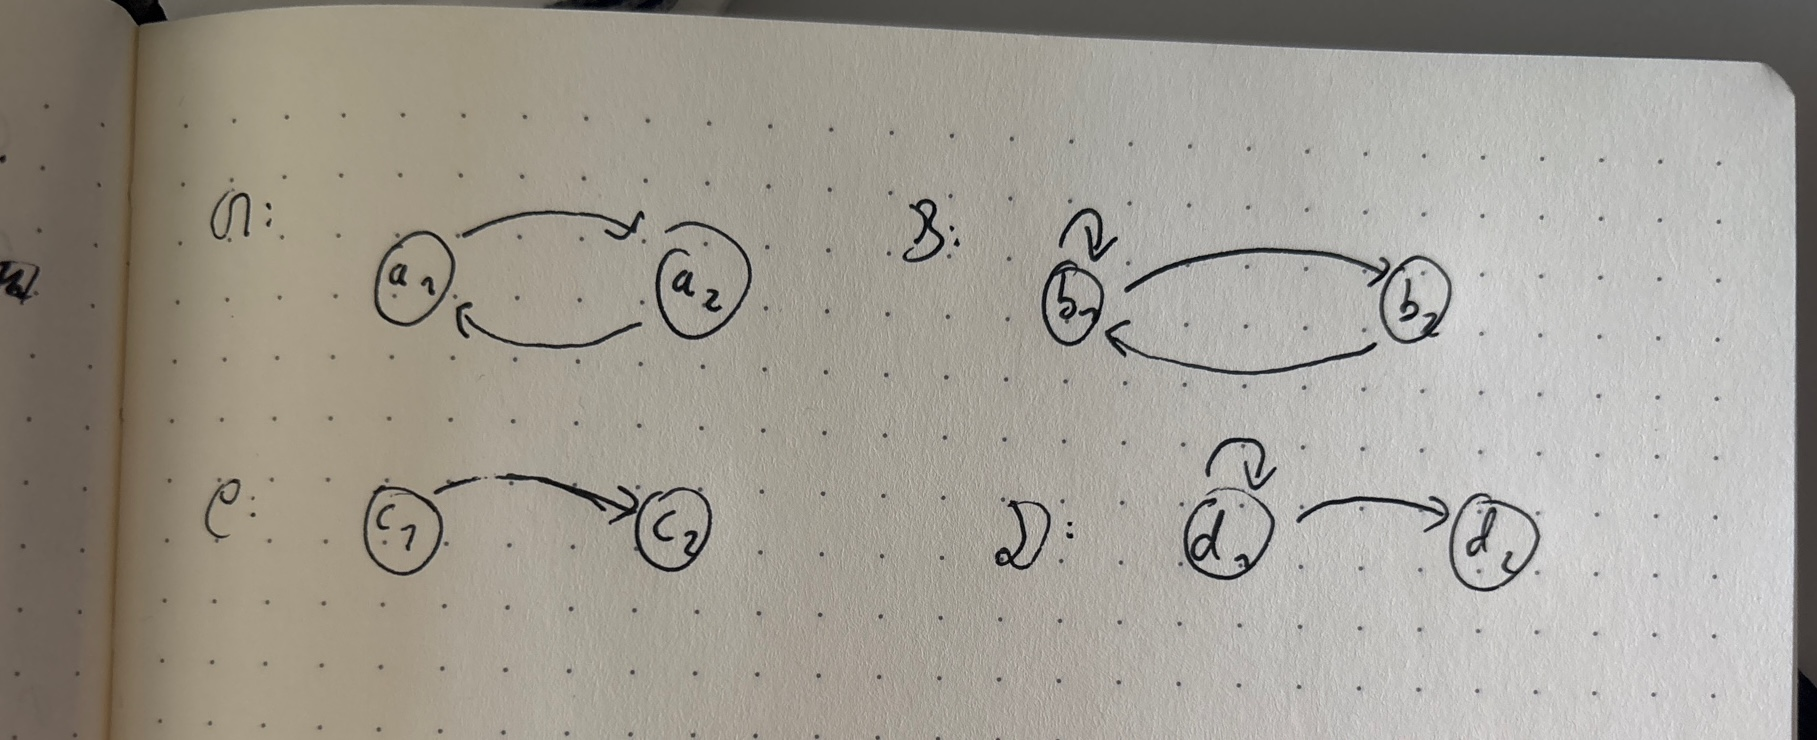
\includegraphics[width=\textwidth]{pictures/totalAndFunctionalStructs}
	\caption{Examples for a total and functional ($\mathfrak A$), a total and not-functional ($\mathfrak B$), a not-total but functional ($\mathfrak C$) and a not-total and not-functional structure ($\mathfrak D$), where $\sigma=\{f/1\}$ and thus $\sigma'=\{R_f/2\}$.}
	\label{fig:totalAndFunctionalStructs}
\end{figure}

To continue, we have to define what it means to be acyclic for a structure with functions.

\begin{definition}[Acyclic, non-relational structures]
	Let $\sigma$ be a signature with function-symbols and $\sigma'$ its encoding as it is defined in section \ref{Sec::NaiveEncodingOfFunctions}.
	Let $\mathfrak C$ be a $\sigma$-structure and $\mathfrak C'$ be its encoding of signature $\sigma'$.
	We then call $\mathfrak C$ acyclic, if $\mathfrak C'$ is acyclic, with respect to acyclicity as it is defined in definition \ref{}.
\end{definition}

We now want to find the equivalence between the existence of an acyclic structure with functions and an encoding of an acyclic structure with the above properties (with respect to homomorphism counting).

\begin{lemma}
	Let $\sigma$ be a signature with function-symbols and $\sigma'$ be the relational encoding of it.
	Let $\mathfrak A$ and $\mathfrak B$ be $\sigma$-structures and $\mathfrak A'$ and $\mathfrak B'$ be their respective encodings of signature $\sigma'$.
	Then the two following statements are equivalent.
	\begin{enumerate}
		\item There exists an acyclic structure $\mathfrak C$ of signature $\sigma$ such that $\hom(\mathfrak C,\mathfrak A)\neq\hom(\mathfrak C,\mathfrak B)$.
		\item There exists an acyclic, total and functional structure $\mathfrak C'$ of signature $\sigma'$ such that $\hom(\mathfrak C',\mathfrak A')\neq \hom(\mathfrak C',\mathfrak B')$.
	\end{enumerate}
\end{lemma}
\begin{proof}
	We begin by proving that \emph{1.} implies \emph{2.}.
	Let $\mathfrak C$ be such a $\sigma$-structure.
	Now let $\mathfrak C'$ be its encoding as a $\sigma'$-structure.
	By definition is $\mathfrak C'$ acyclic and when considering the definition of the encoding, we find that it also has to be total and functional.
	Furthermore we have $\Hom(\mathfrak C,\mathfrak A)=\Hom(\mathfrak C',\mathfrak A')$ and respectively with $\mathfrak B$ and $\mathfrak B'$.
	
	Let $\phi\in\Hom(\mathfrak C,\mathfrak A)$. 
	We show that $\phi\in\Hom(\mathfrak C',\mathfrak A')$.
	Let $(\mathbf xy)\in R^{\mathfrak C'}_f$ for a function-symbol $f\in\sigma$.
	Then by definition of the encoding $f^{\mathfrak C}(\mathbf x)=y$ and then $f^{\mathfrak A}(\phi(\mathbf x))=\phi(f^{\mathfrak C}(\mathbf x))=\phi(y)$.
	Thus we have that $(\phi(\mathbf x)\phi(y))\in R_f^{\mathfrak A'}$, but this is equal to $\phi(\mathbf xy)\in R_f^{\mathfrak A'}$.
	Let $\mathbf x\in R^{\mathfrak C'}$ where $R\neq R_f$ for all function symbols $f\in\sigma$.
	Then we have that $R^{\mathfrak C'}=R^{\mathfrak C}$ and $R^{\mathfrak A}=R^{\mathfrak A'}$. 
	Therefore because $\mathbf x\in R^{\mathfrak C}$, we have $\phi(\mathbf x)\in R^{\mathfrak A}=R^{\mathfrak A'}$. 
	This was to be shown
	
	Let $\phi\in \Hom(\mathfrak C',\mathfrak A')$.
	We show that $\phi\in\Hom(\mathfrak C,\mathfrak A)$.
	Let $\mathbf x\in R^{\mathfrak C}$ for a relational-symbol $R$.
	By the construction of the encoding we know that $R^{\mathfrak C}=R^{\mathfrak C'}$ and $R^{\mathfrak A'}=R^{\mathfrak A}$ and with the same argument as before we can conclude that $\phi(\mathbf x)\in R^{\mathfrak A}$.
	Let $\mathbf x$ and $y$ be such that $f^{\mathfrak C}(\mathbf x)=y$.
	Then by construction we know that $(\mathbf xy)\in R_f^{\mathfrak C'}$.
	Because $\phi$ is a homomorphism we also know that $\phi(\mathbf xy)\in R_f^{\mathfrak A'}$ and because $\mathfrak A'$ is also an encoding we have that $f^{\mathfrak A}(\phi(\mathbf x))=\phi(y)=\phi(f^{\mathfrak C}(\mathbf x))$.
	This was to be shown.
	$\mathfrak A$ and $\mathfrak A'$ can be replaced by $\mathfrak B$ and $\mathfrak B'$, respectively, to get the analogous result for the other structure.
	
	We now show that \emph{2.} implies \emph{1.}.
	Let $\mathfrak C'$ be an acyclic, total and functional $\sigma'$-structure.
	We can now construct a $\sigma$-structure $\mathfrak C$ by decoding $\mathfrak C'$ and will also get that $\Hom(\mathfrak C',\mathfrak A')=\Hom(\mathfrak C,\mathfrak A)$.
	For a relation-symbol $R\in\sigma$ we can define $R^{\mathfrak C}\coloneqq R^{\mathfrak C'}$.
	For a function-symbol $f\in\sigma$ we can define $f^{\mathfrak C}$ as follows: 
	Let $f$ be of arity $n$. Then for a $n$-ary tuple $\mathbf x$ there must be a $y$ such that $(\mathbf xy)\in R_f^{\mathfrak C'}$ because $\mathfrak C'$ is total and there must be exactly one such $y$ because $\mathfrak C'$ is functional.
	Therefore we define $f^{\mathfrak C}(\mathbf x)=y$.
	The claim that the sets of homomorphisms is equal can be verified using exactly the same arguments as in the analogous proof of the other direction.
\end{proof}

We can now continue to put this in relation to the statement regarding RCR.
We have that naive RCR distinguishes two $\sigma$-structures $\mathfrak A$ and $\mathfrak B$ if, and only if, RCR distinguishes the encodings $\mathfrak A'$ and $\mathfrak B'$ of signature $\sigma'$.
Due to the results of \cite{scheidt2025ColorRefinement} this is the case if, and only if, there is an acyclic $\sigma'$-structure $\mathfrak C'$ such that $\hom(\mathfrak C',\mathfrak A')\neq\hom(\mathfrak C',\mathfrak B')$.
We would like to achieve the result that this is equivalent to there being an acyclic $\sigma$ structure that distinguishes $\mathfrak A$ and $\mathfrak B$ by homomorphism count (however this will not be the case).
By the above lemma, this is equivalent to there being an acyclic, total and functional $\sigma'$-structure $\mathfrak C''$ that distinguishes $\mathfrak A'$ and $\mathfrak B'$ by homomorphism count.
Our goal will therefore be, to study the relationship between the two following statements.
\begin{enumerate}
	\item There is an acyclic $\sigma'$-structure $\mathfrak C'$ such that $\hom(\mathfrak C',\mathfrak A')\neq\hom(\mathfrak C',\mathfrak B')$.
	\item There is an acyclic, total and functional $\sigma'$-structure $\mathfrak C''$ such that $\hom(\mathfrak C'',\mathfrak A')\neq\hom(\mathfrak C'',\mathfrak B')$.
\end{enumerate}

It is obvious that \emph{2.} implies \emph{1.}, however the other direction will not hold in general.
In fact, we will be able to construct a functional structure from $\mathfrak C'$, but totality will not be able to be constructed.
We will in the following prove the former claim and then show the latter claim, using a family of counterexamples.

\begin{lemma}
	Let $\mathfrak A$ and $\mathfrak B$ be structures of signature $\sigma$ and $\mathfrak A'$, $\mathfrak B'$ and $\sigma'$ the respective encodings.
	If there is an acyclic structure $\mathfrak C'$ of signature $\sigma'$ with $\hom(\mathfrak C',\mathfrak A')\neq\hom(\mathfrak C',\mathfrak B')$, then we can construct a functional, acyclic structure $\mathfrak C''$ of signature $\sigma'$ such that $\hom(\mathfrak C'',\mathfrak A')=\hom(\mathfrak C',\mathfrak A')$ and $\hom(\mathfrak C'',\mathfrak B')=\hom(\mathfrak C',\mathfrak B')$.
\end{lemma}
\begin{proof}
	The proof for the above lemma will work as follows.
	If $\mathfrak C'$ is not functional, then there is a function-symbol $f\in\sigma$ and two different tuples $(\mathbf xy),(\mathbf xz)\in R^{\mathfrak C'}_f$, we call this a collision.
	We will give a procedure, to iteratively remove such collisions.
	The procedure will reduce the number of elements by one, will keep the acyclicity property and will result in a structure with the same amount of homomorphisms to $\mathfrak A'$ and $\mathfrak B'$.
	Thus, by continuously applying that procedure to all collisions, we will get $\mathfrak C''$.
	The algorithm must terminate, as the number of elements strictly decreases and we only consider finite structures.
	
	The remainder of this proof will be dedicated to describing the procedure and proving the above claims.
	Assume that there is a function symbol $f\in \sigma$ and two different tuples $(\mathbf x y),(\mathbf x z)\in R_f^{\mathfrak C'}$. 
	Our goal will be to construct a structure $\mathfrak C''$ of signature $\sigma'$ without this particular collision and with the following properties:
	\begin{itemize}
		\item[a.] $\Vert \mathfrak C'' \Vert = \Vert \mathfrak C'\Vert -1$
		\item[b.] $\mathfrak C''$ is acyclic
		\item[c.] $\hom(\mathfrak C'',\mathfrak A')=\hom(\mathfrak C',\mathfrak A')$ and $\hom(\mathfrak C'',\mathfrak B')=\hom(\mathfrak C',\mathfrak B')$.
	\end{itemize}
	We define the function $\chi : \mathbf{C'}\to\mathbf{C''}$ which will map tuples of $\mathfrak C'$ to tuples of $\mathfrak C''$ with the same arity.
	Concretely, for an arbitrary tuple $\mathbf c\in \mathbf{C'}$ of arity $k$ and for every $i\in[k]$, we have
	$$\chi(\mathbf c)_i \coloneqq \begin{cases}
		c_i & \text{if } c_i\notin \{y,z\} \\
		v_{y,z} & \text{if } c_i \in \{y,z\}
	\end{cases}$$
	for a new element $v_{y,z}$.
	In words, we replace every occurrence of $y$ and $z$ by $v_{y,z}$, while letting everything else stay the same.
	Now we can define 
	$$\mathfrak C'' \coloneqq ((C' \setminus \{y,z\})\cup \{v_{y,z}\}, \sigma),$$
	where for all $R\in\sigma'$ we have $R^{\mathfrak C''}\coloneqq \{\chi(\mathbf c) : \mathbf c\in R^{\mathfrak C'}\}$.
	We will now proceed by proving the above properties.
	
	\paragraph{Property a.:}
	This property follows directly from the definition of $C''$.
	We have $y\neq z$, $y,z\in C'$ and thus $\vert C'\setminus \{y,z\}\vert = \vert C'\vert -2$.
	Furthermore, we have $v_{y,z}\notin C'$ and therefore $\vert (C'\setminus \{y,z\})\cup \{v_{y,z}\}\vert = \vert C' \vert -1$.
	This was to be shown.
	
	\paragraph{Property b.:}
	To show that $\mathfrak C''$ is acyclic, we first will define an undirected graph $J''$, will prove that it is connected and cycle free, thus a tree, and that it fulfils the join tree property for $\mathfrak C''$.
	By the assumption we know that $\mathfrak C'$ is acyclic and thus has a join tree $J'$.
	We further notice that $\mathbf{C''}=\{\chi(\mathbf c) : \mathbf c\in \mathbf{C'}\}$.
	Now we define $V(J'')\coloneqq \mathbf{C''}$ and $E(J'')\coloneqq \{\{\chi(\mathbf u),\chi(\mathbf v)\} : \{\mathbf u,\mathbf v\}\in E(J')\}$.
	
	\begin{claim}
		$J''$ is connected.
	\end{claim}
	\begin{proof}
		Consider $\mathbf u,\mathbf v\in V(J'')$.
		Then there are $\mathbf a,\mathbf b\in V(J')$, such that $\chi(\mathbf a)=\mathbf u$ and $\chi(\mathbf b)=\mathbf v$.
		By assumption, $J'$ is a tree, so there are $\mathbf a_0,\mathbf a_1,\dots,\mathbf a_k$ with $\mathbf a_0=\mathbf a$, $\mathbf a_k=\mathbf b$ and $\{\mathbf a_{i-1},\mathbf a_{i}\}\in E(J')$ for all $i\in [k]$.
		By definition, we have $\chi(\mathbf a_0),\chi(\mathbf a_1),\dots,\chi(\mathbf a_k)\in V(J'')$ with $\chi(\mathbf a_0)=\chi(\mathbf a)=\mathbf u$, $\chi(\mathbf a_k)=\chi(\mathbf b)=\mathbf v$ and $\{\chi(\mathbf a_{i-1}),\chi(\mathbf a_i)\}\in E(J'')$ for all $i\in[k]$.
		Thus $\mathbf u$ and $\mathbf v$ are connected.
	\end{proof}
	
	In the following, for an arbitrary $e \in C'$, we define the set $V_e\coloneqq \{\mathbf c\in V(J') : e\in \mathbf c\}$.
	One can see that $V(J'_e)=V_e$, where $J'_e$ is the subgraph of $J'$, induced by all elements containing $e$.
	
	\begin{claim}
		$J''$ is cycle-free.
	\end{claim}
	\begin{proof}
		Assume that there were $\mathbf u_0,\mathbf u_1,\dots,\mathbf u_k\in V(J'')$ with $\{\mathbf u_{i-1},\mathbf u_i\}\in E(J'')$ for all $i\in [k]$ and $\{\mathbf u_k,\mathbf u_0\}\in E(J'')$.
		We now define directed edges such that $e_0=(\mathbf u_0,\mathbf u_1)$, $e_1=(\mathbf u_1,\mathbf u_2)$, $\dots$, $e_k=(\mathbf u_k,\mathbf u_0)$, therefore we have $e_i=(\mathbf u_i, \mathbf u_{\ipo k})$.
		For every edge $e_i$ choose two elements $\mathbf a_i,\mathbf b_i\in V(J')$ such that $\{\mathbf a_i,\mathbf b_i\}\in E(J')$, $\chi(\mathbf a_i)=\mathbf u_i$ and $\chi(\mathbf b_i)=\mathbf u_{\ipo k}$.
		These elements must exist by the definition of $E(J'')$.
		
		We now prove that there exists a cycle in $J'$, which would contradict our assumption of $J'$ being a join tree for $\mathfrak C'$.
		To show this, we prove that for all $i\in\{0\}\cup[k]$, the elements $\mathbf b_i$ and $\mathbf a_{\ipo k}$ are connected in $J'$.
		We see that $\chi(\mathbf b_i)=\mathbf u_{\ipo k} = \chi(\mathbf a_{\ipo k})$.
		
		If there is a $c\in \set(\mathbf u_{\ipo k})$ with $c\neq v_{y,z}$, then by definition of $\chi$, we have $c\in \set(\mathbf b_i)\cap \set(\mathbf a_{\ipo k})$.
		Therefore $\mathbf b_i,\mathbf a_{\ipo k}\in V_c$ and because $J'$ is a join tree, $\mathbf b_i$ and $\mathbf a_{\ipo k}$ have to be connected.
		
		If $\set(\mathbf u_{\ipo k})=\{v_{y,z}\}$, we have four possible cases.
		If $y\in \set(\mathbf b_i)\cap \set(\mathbf a_{\ipo k})$ or $z\in \set(\mathbf b_i)\cap \set(\mathbf a_{\ipo k})$, then we can do the same as before by setting $c=y$ or $c=z$, respectively.
		Otherwise we have $y\in\set(\mathbf b_i)$ and $z\in \set(\mathbf a_{\ipo k})$, or $z\in\set(\mathbf b_i)$ and $y\in \set(\mathbf a_{\ipo k})$.
		We will only consider the former option, as the latter can be proven analogously.
		From our beginning assumption we know that $(\mathbf xy),(\mathbf xz)\in R_f$. Choose some $x\in\mathbf x$, and $(\mathbf xy),(\mathbf xz)\in V_x$ follows.
		Furthermore, we have $\mathbf b_i,(\mathbf xy)\in V_y$ and $\mathbf a_{\ipo k},(\mathbf xz)\in V_z$.
		Since $J'$ is a join tree, we thus know that $\mathbf b_i$ is connected with $(\mathbf xy)$, which in turn is connected with $(\mathbf xz)$, which again is connected with $\mathbf a_{\ipo k}$.
		Therefore $\mathbf b_i$ and $\mathbf a_{\ipo k}$ are connected.
		
		Thus we have found a cycle in $J'$, which is a contradiction to it being a join tree.
		Therefore our assumption of the existence of the elements $\mathbf u_0,\mathbf u_1,\dots,\mathbf u_k$ has to be false.
	\end{proof}
	
	The last missing piece to prove the acyclicity of $\mathfrak C''$ is to show that $J''$ fulfils the join tree property.
	That is, for any $c\in C''$, the set $\{\mathbf c\in V(J'') : c\in\set(\mathbf c)\}$ induces a connected subgraph of $J''$.
	
	\begin{claim}
		$J''$ is a valid join tree.
	\end{claim}
	\begin{proof}
		Consider any $c\in C''$ and two elements $\mathbf u$ and $\mathbf v$ from the set $S\coloneqq \{\mathbf c \in V(J'') : c\in \set(\mathbf c)\}$.
		We show that there is a path from $\mathbf u$ to $\mathbf v$ in $S$.
		If $v\neq v_{y,z}$, then $v\in C'$, thus consider $V_c$.
		By definition there are $\mathbf a,\mathbf b\in V_c$ such that $\chi(\mathbf a)=\mathbf u$ and $\chi(\mathbf b)=\mathbf v$.
		Because $J'$ is a join tree, $V_c$ must induce a connected subtree.
		Thus there must be $\mathbf a_0,\dots,\mathbf a_k\in V_c$ such that $\mathbf a_0=\mathbf a$, $\mathbf a_k=\mathbf b$ and $\{\mathbf a_{i-1},\mathbf a_i\}\in E(J')$ for all $i\in [k]$.
		By definition we then get, that there must be $\chi(\mathbf a_0),\chi(\mathbf a_k)\in S$ and we get $\chi(\mathbf a_0)=\chi(\mathbf a)=\mathbf u$, $\chi(\mathbf a_k)=\chi(\mathbf b)=\mathbf v$ and $\{\chi(\mathbf a_{i-1},\mathbf a_i)\}\in E(J''))$ for all $i\in[k]$.
		Therefore, $\mathbf u$ and $\mathbf v$ are connected in $S$.
		
		If $v=v_{y,z}$, we again define $\mathbf a,\mathbf b\in V(J')$ such that $\chi(\mathbf a)=\mathbf u$ and $\chi(\mathbf b)=\mathbf v$.
		If $\mathbf a,\mathbf b\in V_y$ or $\mathbf a,\mathbf b\in V_z$, then we can proceed exactly as in the former case with $v=y$ or $v=z$, respectively.
		If that is not the case, then either $\mathbf a\in V_y and \mathbf b\in V_z$, or the other way round.
		We will only prove the former case, as the latter case can proven analogously.
		Since the following will depend on it, we will now prove the following equality: $S=\{\chi(\mathbf c) : \mathbf c\in V_y\}\cup \{\chi(\mathbf c) : \mathbf c\in V_z\}$.
		
		$\supseteq$:
		Let $\mathbf u \in \{\chi(\mathbf c) : \mathbf c\in V_y\}\cup \{\chi(\mathbf c) : \mathbf c\in V_z\}$.
		We then get that $\mathbf u = \chi(\mathbf a)$ for an $\mathbf a\in V(J')$.
		From the definition it follows that $y\in \set(\mathbf a)$ or $z\in \set(\mathbf a)$ has to hold.
		Thus we get that $v_{y,z}\in \set(\chi(\mathbf a))=\set(\mathbf u)$ and therefore $\mathbf u\in S$ has to hold.
		
		$\subseteq$:
		Let $\mathbf u\in S$, then $v_{y,z}\in \set(\mathbf u)$ follows.
		By definition there must exist an $\mathbf a \in V(J')$ such that $\chi(\mathbf a)=\mathbf u$ and $y\in \set(\mathbf a)$ or $z\in \set(\mathbf a)$ has to hold.
		Thus we get $\chi(\mathbf a)=\mathbf u\in \{\chi(\mathbf c) : \mathbf c\in V_y\}\cup \{\chi(\mathbf c) : \mathbf c\in V_z\}$
		
		It is obvious that $(\mathbf xy)\in V_y$ and $(\mathbf xz)\in V_z$.
		We now get a path in $V_y$ with the elements $\mathbf a_0,\dots,\mathbf a_k\in V_b$ such that $\mathbf a_0=\mathbf a$, $\mathbf a_k=(\mathbf xy)$ and $\{\mathbf a_{i-1},\mathbf a_i\}\in E(J')$ for all $i\in [k]$.
		We also get a path in $V_z$ with the elements $\mathbf b_0,\dots,\mathbf b_\ell\in V_z$ such that $\mathbf b_0=(\mathbf xz)$, $\mathbf b_\ell = \mathbf b$ and $\{\mathbf b_{i-1},\mathbf b_i\}\in E(J')$.
		Therefore with the above equation, we have two paths in $S$: $\chi(\mathbf a_0),\dots,\chi(\mathbf a_k)$ and $\chi(\mathbf b_0),\dots,\chi(\mathbf b_\ell)$, where $\chi(\mathbf a_0)=\mathbf u$ and $\chi(\mathbf b_\ell)=\mathbf v$.
		Now we have that $\chi(\mathbf a_k)=\chi((\mathbf xy))=(\mathbf x'v_{y,z})=\chi((\mathbf xz))=\chi(\mathbf b_0)$.
		Therefore, we get one path from $\mathbf u$ to $\mathbf v$ in $S$.
	\end{proof}
	
	\paragraph{Property c.:}
	To show that $\hom(\mathfrak C'',\mathfrak A')=\hom(\mathfrak C',\mathfrak A')$ and $\hom(\mathfrak C'',\mathfrak B')=\hom(\mathfrak C',\mathfrak B')$, we will give a mapping $\pi : \Hom(\mathfrak C',\mathfrak A')\to\Hom(\mathfrak C'',\mathfrak A')$ from homomorphisms from $\mathfrak C'$ to $\mathfrak A'$ to homomorphisms from $\mathfrak C''$ to $\mathfrak A'$.
	We will then show that $\pi$ is a bijection, from which follows that both sets have the same cardinality, which then proves the claim for $\mathfrak A'$.
	For $\mathfrak B'$, the prove is completely analogous, which is why it will be omitted.
	Let $\phi\in \Hom(\mathfrak C',\mathfrak A')$.
	We now define $\phi'\coloneqq \pi(\phi)$ as
	$$
	\phi'(x)=
	\begin{cases}
		\phi(x) & \text{if } x\neq v_{y,z} \\
		\phi(y) & \text{if } x = v_{y,z}.
	\end{cases}
	$$
	In the following we will be using that for any $\phi\in\Hom(\mathfrak C',\mathfrak A')$, we have that $\phi(y)=\phi(z)$.
	Otherwise, from $(\mathbf xy),(\mathbf xz)\in R_f^{\mathfrak C'}$, it follows that $(\phi(\mathbf x)\phi(y)),(\phi(\mathbf x)\phi(z))\in R_f^{\mathfrak A'}$ for two different tuples $(\phi(\mathbf x)\phi(y))$ and $(\phi(\mathbf x)\phi(z))$.
	However, this would contradict that, by definition of the encoding, $\mathfrak A'$ is functional.
	
	\begin{claim}
		For all $\phi\in \Hom(\mathfrak C',\mathfrak A')$, we have $\pi(\phi)\in\Hom(\mathfrak C'',\mathfrak A')$.
	\end{claim}
	\begin{proof}
		Let $\phi\in\Hom(\mathfrak C',\mathfrak A')$ and $\phi'\coloneqq \pi(\phi)$.
		Consider a relation-symbol $R$ and a tuple $\mathbf c \in R^{\mathfrak C''}$.
		If $v_{y,z}\notin\set(\mathbf c)$, then $\chi(\mathbf c)=\mathbf c$, $\phi(\mathbf c)=\phi'(\mathbf c)$ and $\mathbf c\in R^{\mathfrak C'}$ follows.
		Then we get $\phi(\mathbf c)\in R^{\mathfrak A'}$ and further $\phi'(\mathbf c)\in R^{\mathfrak A'}$.
		
		If $v_{y,z}\in\set(\mathbf c)$, then there exists a $\mathbf c'\in R^{\mathfrak C'}$ such that $\chi(\mathbf c')=\mathbf c$. 
		We thus get $\phi(\mathbf c')\in R^{\mathfrak A'}$.
		We also have that $\phi(\mathbf c')=\phi'(\mathbf c)$, because for all $x \in \set(\mathbf c)\setminus \{v_{y,z}\}$, we also have $x\in\set(\mathbf c')$ and $\phi(x)=\phi'(x)$.
		For $v_{y,z}$ we have that $\phi'(v_{y,z})=\phi(y)=\phi(z)$.
		Therefore, $\phi'(\mathbf c)\in R^{\mathfrak A'}$ follows, which was to be shown.
	\end{proof}
	
	This shows that $\pi$ is correctly defined as a mapping between homomorphisms.
	The two following proofs will show that $\pi$ is bijective.
	
	\begin{claim}
		$\pi$ is injective.
	\end{claim}
	\begin{proof}
		Let $\phi_1,\phi_2\in\Hom(\mathfrak C',\mathfrak A')$, $\phi_1\neq\phi_2$ and define $\phi_1'\coloneqq \pi(\phi_1)$ and $\phi_2'\coloneqq \pi(\phi_2)$.
		Our goal is to show that $\phi_1'\neq \phi_2'$.
		There has to be a $u\in C'$ such that $\phi_1(u)\neq\phi_2(u)$, otherwise they would be the same function.
		We now do a case distinction.
		
		\emph{Case 1:} $u\notin\{y,z\}$. Then we have
		$$\phi_1'(u)=\phi_1(u)\neq \phi_2(u)=\phi_2'(u).$$
		\emph{Case 2:} $u\in \{y,z\}$. Then we have 
		$$\phi_1'(v_{y,z})=\phi_1(y)=\phi_1(z)=\phi_1(u)\neq \phi_2(u)=\phi_2(z)=\phi_2(y)=\phi_2'(v_{y,z}).$$
		In both cases we thus have found an element that gets mapped differently, thus $\phi_1'\neq\phi_2'$ must follow.
	\end{proof}
	
	\begin{claim}
		$\pi$ is surjective.
	\end{claim}
	\begin{proof}
		Let $\phi'\in\Hom(\mathfrak C'',\mathfrak A')$.
		We now construct a $\phi\in\Hom(\mathfrak C',\mathfrak A')$ such that $\pi(\phi)=\phi'$.
		We define
		$$
		\phi(x)=
		\begin{cases}
			\phi'(x) & \text{if } x \notin \{y,z\} \\
			\phi'(v_{y,z}) & \text{if } x \in \{y,z\}.
		\end{cases}
		$$
		Using that $\psi(y)=\psi(z)$ for all $\psi\in\Hom(\mathfrak C',\mathfrak A')$, it can easily be verified that $\pi(\phi)=\phi'$.
		We now only have to show that $\phi\in\Hom(\mathfrak C',\mathfrak A')$. 
		Let $\mathbf c\in R^{\mathfrak C'}$ for a relation-symbol $R$.
		We now define $\mathbf c'\coloneqq \chi(\mathbf c)$ and get by construction that $\mathbf c'\in R^{\mathfrak C''}$.
		Because we know that $\phi'$ is a homomorphism, it follows that $\phi'(\mathbf c')\in R^{\mathfrak A'}$.
		But since $\phi'(a)=\phi(a)$ for all $a\notin \{y,z,v_{y,z}\}$ and $\phi'(v_{y,z})=\phi(y)=\phi(z)$, it follows that $\phi'(\mathbf c')=\phi(\mathbf c)$.
		Therefore $\phi(\mathbf c)\in R^{\mathfrak A'}$.
	\end{proof}
	
	We now have proved all properties.
	Therefore we have devised a procedure, to iteratively construct a functional, acyclic structure, that divides $\mathfrak A'$ and $\mathfrak B'$ by homomorphism count.
\end{proof}

\section {Relational Colour Refinement for symmetric structures}

One very interesting subclass of relational structures is the class of symmetric structures.
A special case of these are for example undirected graphs, as their edge relations are symmetric.
This notion of symmetry can be generalized to any relational signature.

\begin{definition}[Symmetric Structures]
	Let $\sigma$ be a relational signature.
	A structure $\mathfrak A$ of signature $\sigma$ is a symmetric structure, if for every relation and every tuple in those relations, the order of the elements is irrelevant.
	This means, that every relation $R$ with arity $k$ is a subset of all possible subsets of $A$ with exactly $k$ elements.
	Formally, we have
	$$R\subseteq \binom{A}{k}.$$
\end{definition}
An equivalent characterisation uses the symmetric groups $\mathcal S_k$.
We call a $\sigma$ structure $\mathfrak A$ symmetric, if for every $R\in \sigma$ of arity $k$, every $k$-tuple $\mathbf x=(x_1,x_2,\dots,x_k)\in R^{\mathfrak A}$ and every $k$-permutation $\pi\in \mathcal S_k$, we have that
$$(x_{\pi(1)},x_{\pi(2)},\dots,x_{\pi(k)})\in R^{\mathfrak A}.$$
In the following, we will use $\pi(\mathbf x)$ as a shorthand notation for $(x_{\pi(1)},x_{\pi(2)},\dots,x_{\pi(k)})$.

As symmetric structures are a subset of relational structures, the results from \cite{scheidt2025ColorRefinement} obviously apply to them.
Thus, we have that the following three statements are equivalent for two symmetric $\sigma$ structures $\mathfrak A$ and $\mathfrak B$:
\begin{enumerate}
	\item $\RCR$ distinguishes $\mathfrak A$ and $\mathfrak B$.
	\item There exists a sentence $\phi\in\GFC$, such that $\mathfrak A\models \phi$ and $\mathfrak B\not\models \phi$.
	\item There exists an acyclic $\sigma$ structure $\mathfrak C$, such that $\hom(\mathfrak C,\mathfrak A)\neq\hom(\mathfrak C,\mathfrak B)$.
\end{enumerate}
However, as we restricted the class of structures for $\mathfrak A$ and $\mathfrak B$, this poses the question, whether the same can be done to the acyclic structures.
Concretely, we want to investigate, whether the first statement is also equivalent to there being an acyclic, symmetric $\sigma$ structure, such that it has a different homomorphism count to $\mathfrak A$ than to $\mathfrak B$.

As we will prove in the following, it is indeed the case that we can restrict the class of acyclic structures to only include structures that acyclic and symmetric.
However, before we prove this, we have to show a lemma which will be used in the proof.
As a reminder on notation, for a $k$-tuple $\mathbf x=(x_1,x_2,\dots,x_k)$ a homomorphism $\phi$ and a permutation $\pi$ we write $\phi(\mathbf x)$ for $(\phi(x_1),\phi(x_2),\dots,\phi(x_k))$ and $\pi(\mathbf x)$ for $(x_{\pi(1)},x_{\pi(2)},\dots,x_{\pi(k)})$.
\begin{lemma}
	Let $\pi\in\mathcal S_k$, $\phi$ be a homomorphism, $R$ a $k$-ary relation and $\mathbf x\in R$.
	Then $\phi(\pi(\mathbf x))=\pi(\phi(\mathbf x))$.
\end{lemma}
\begin{proof}
	We prove this by contradiction.
	Assume the contrary.
	Then there exists an $i\in[k]$, such that $\phi(\pi(\mathbf x))_i\neq \pi(\phi(\mathbf x))_i$.
	Note that the definitions of $\phi(\pi(\mathbf x))$ and $\pi(\phi(\mathbf x))$ are 
	$$\phi(\pi(\mathbf x)) = (\phi(x_{\pi(1)}), \phi(x_{\pi(2)}),\dots,\phi(x_{\pi(k)}))$$
	and
	$$\pi(\phi(\mathbf x)) = (\phi(\mathbf x)_{\pi(1)},\phi(\mathbf x)_{\pi(2)},\dots,\phi(\mathbf x)_{\pi(k)}).$$
	From these, we directly get
	$$\phi(\pi(\mathbf x))_i=\phi(x_{\pi(i)})=(\phi(x_1),\phi(x_2),\dots,\phi(x_2))_{\pi(i)}=\phi(\mathbf x)_{\pi(i)}=\pi(\phi(\mathbf x))_i.$$
	Contradiction!
	Therefore the lemma must hold.
\end{proof}
We now prove the above claim:
\begin{theorem}
	Let $\sigma$ be a relational signature and $\mathfrak A$ and $\mathfrak B$ be two $\sigma$ structures.
	Then the following two statements are equivalent:
	\begin{enumerate}
		\item $\RCR$ distinguishes $\mathfrak A$ and $\mathfrak B$.
		\item There exists an acyclic, symmetric $\sigma$ structure $\mathfrak C$ with $\hom(\mathfrak C,\mathfrak A)\neq \hom(\mathfrak C,\mathfrak B)$.
	\end{enumerate}
\end{theorem}
\begin{proof}
	We first prove that \textit{2.} implies \text{1.}.
	Let $\mathfrak C$ be a acyclic, symmetric $\sigma$ structure with $\hom(\mathfrak C,\mathfrak A)\neq\hom(\mathfrak C,\mathfrak B)$.
	As $\mathfrak C$ is acyclic, we can apply \ref{} and get that $\RCR$ must distinguish $\mathfrak A$ and $\mathfrak B$.
	
	We now prove that \textit{1.} implies \textit{2.}.
	Assume that $\RCR$ distinguishes $\mathfrak A$ and $\mathfrak B$.
	From \ref{} we know that there exists an acyclic structure $\mathfrak C'$ with $\hom(\mathfrak C',\mathfrak A)\neq \hom(\mathfrak C',\mathfrak B)$.
\end{proof}





\section{Conclusion}

In this thesis, we presented the results of Scheidt and Schweikardt \cite{scheidt2025ColorRefinement} and discussed how they can be extended for the use with non-relational structures.
We presented two possible ways on how non-relational structures can be encoded as relational structures and investigated the logical and combinatorial characterisations.
Naive Relational Colour Refinement, where a function is directly interpreted as a relation, is characterised by the logic $\mathsf{nfGF}(\mathsf C)$, which uses function symbols like relation symbols.
By using the transitive expansion of a function as its encoding, we can allow arbitrarily many function applications, with a bound on the number of alternations. 
This notion is captured by the logic $\GFC_k$.
However, while we find a logical characterisation, the combinatorial characterisation is not possible.
We showed that the existence of an acyclic, total, functional relational structure that distinguishes two encoded structures by homomorphism count is equivalent to the existence of a non-relational structure that also distinguishes the structures.
But while it is possible to construct a functional structure, it is not possible to enforce totality.
This then lead us to the question of investigating restrictions of the class of structures and for which restrictions the characterisation by homomorphism counting remains.
Aside from the negative result in that regard for total structures, we showed that it is possible to restrict the class to symmetric structures.

There are multiple questions that are still unanswered.
\begin{itemize}
	\item When characterising $\RCR_k$ logically, we were able to show that the number of applications of a single function symbol does not need a bound.
	The same was not done for the alternation depth.
	One interesting question would be to investigate, whether it is possible to only consider the transitive expansion up to a certain alternation depth $d$.
	Furthermore, would it then be possible to allow any alternation depth in a formula to characterise this algorithm?
	The result would then be that $\GFC$ with the standard definition atomic formulae would characterise $\RCR$ over non-relational structures.
	\item Our two algorithms operate on different classes of structures.
	While nRCR is defined for any structure, $\RCR_k$ only works for structures over signatures with relation and unary function symbols.
	It is not clear, whether the used approach can be adapted for functions with arity $\geq 2$.
	However, an iterative colouring algorithm that is stronger than nRCR but still works on any structure is desirable.
	\item We have considered two possible restrictions on the class of relational structures for characterisation by homomorphism counting.
	This poses the question, which other restriction could be characterised this way.
\end{itemize}




\clearpage

\bibliographystyle{plainurl}
\bibliography{references.bib}





\end{document}





